\documentclass[preprint,12pt]{elsarticle}

\usepackage[hidelinks]{hyperref}
\usepackage{graphicx}
\usepackage{subcaption}
\usepackage{amssymb}
\usepackage{amsmath}
\usepackage{multirow}
\usepackage[utf8]{inputenc}
\usepackage{ifthen}
\usepackage{cleveref}
\usepackage{listings}
\usepackage[ruled,vlined]{algorithm2e}
\usepackage{booktabs}

% For the TODOs
\usepackage{xcolor}
\usepackage{xargs}
\usepackage[colorinlistoftodos,textsize=footnotesize]{todonotes}
\newcommand{\todoin}{\todo[inline]}
% from here: https://tex.stackexchange.com/questions/9796/how-to-add-todo-notes
\newcommandx{\unsure}[2][1=]{\todo[linecolor=red,backgroundcolor=red!25,bordercolor=red,#1]{#2}}
\newcommandx{\change}[2][1=]{\todo[linecolor=blue,backgroundcolor=blue!25,bordercolor=blue,#1]{#2}}
\newcommandx{\info}[2][1=]{\todo[linecolor=OliveGreen,backgroundcolor=OliveGreen!25,bordercolor=OliveGreen,#1]{#2}}

%Boldtype for greek symbols
\newcommand{\teng}[1]{\ensuremath{\boldsymbol{#1}}}
\newcommand{\ten}[1]{\ensuremath{\mathbf{#1}}}

\lstset{language=Python,
  basicstyle=\ttfamily\bfseries\small,
  commentstyle=\color{red}\itshape,
  stringstyle=\ttfamily\color{green!50!black},
  showstringspaces=false,
  keywordstyle=\color{blue}\bfseries}

\newcommand{\code}[1]{\lstinline{#1}}
\newcommand{\codek}[1]{\lstinline[keywordstyle=\color{black}]{#1}}

\DeclareMathOperator*{\argmax}{arg\,max}
\DeclareMathOperator*{\argmin}{arg\,min}
%
\usepackage{lineno}
\usepackage{tikz}
\usetikzlibrary{arrows.meta, patterns}
\usetikzlibrary{shapes, calc,quotes,angles}
\tikzset{%
  >={Latex[width=2mm,length=2mm]},
  % Specifications for style of nodes:
  base/.style = {
    rectangle, rounded corners, draw=black, minimum width=4cm, minimum
    height=1cm, text centered, font=\sffamily},
  decision/.style = {
    diamond, draw, rounded corners, fill=blue!20, minimum width=3cm, minimum height=0.5cm, text centered, font=\sffamily},
  activityStarts/.style = {base, fill=blue!30},
  startstop/.style = {base, fill=red!30},
  activityRuns/.style = {base, fill=green!30},
  process/.style = {
    base, minimum width=2.5cm, fill=orange!15, font=\ttfamily},
}
\journal{}
%
\begin{document}

% set showimages to 0 to shutoff all the images
\def\showimages{1}
%%%%%%%%%%%%%%%%%%%%%%%%%%%%%%5

\begin{frontmatter}

  \title{Algorithms for uniform particle initialization in domains
  with complex boundaries}

  \author[IITB]{Pawan Negi\corref{cor1}}
  \ead{pawan.n@aero.iitb.ac.in}
  \author[IITB]{Prabhu Ramachandran}
  \ead{prabhu@aero.iitb.ac.in}
\address[IITB]{Department of Aerospace Engineering, Indian Institute of
  Technology Bombay, Powai, Mumbai 400076}

\cortext[cor1]{Corresponding author}

\begin{abstract}

  Accurate mesh-free simulation of fluid flows involving complex boundaries
  requires that the boundaries be captured accurately in terms of particles.
  In the context of incompressible/weakly-compressible fluid flow, the SPH
  method is more accurate when the particle distribution is uniform. Hence,
  for time-accurate simulation of flow in the presence of complex boundaries
  one must have both an accurate boundary discretization and a uniform
  distribution of particles to initialize the simulation. This process of
  obtaining an initial uniform distribution of particles is called ``particle
  packing''. In this paper, we compare and implement various particle packing
  algorithms present in the literature. We propose an improved SPH-based
  algorithm which produces uniform particle distributions of both the fluid
  and solid domains in two and three dimensions. We demonstrate the accuracy of
  the new algorithm by constructing some challenging geometries. The
  implementation of the algorithm is open source, and the manuscript is fully
  reproducible.
\end{abstract}

\begin{keyword}
%% keywords here, in the form: keyword \sep keyword
{Particle packing}, {complex geometry}, {pre-processing}, {smoothed particle
hydrodynamics}

%% MSC codes here, in the form: \MSC code \sep code
%% or \MSC[2008] code \sep code (2000 is the default)

\end{keyword}

\end{frontmatter}

% \linenumbers
%% MSC codes here, in the form: \MSC code \sep code
%% or \MSC[2008] code \sep code (2000 is the default)
\section*{Program summary}
\noindent
\textit{Program title}: SPHGeom

\noindent
\textit{Licensing provisions}: BSD 3-Clause

\noindent
\textit{Programming language}: Python

\begin{sloppypar}
  \noindent
  \textit{External routines/libraries}: PySPH
  (\url{https://github.com/pypr/pysph}), matplotlib
  (\url{https://pypi.org/project/matplotlib/}), automan
  (\url{https://pypi.org/project/automan/}),
  ParaView(\url{https://www.paraview.org/download/}).
\end{sloppypar}
\noindent
\textit{Nature of problem}: Particle methods require that complex geometry be
accurately represented when discretized with particles. The particles should
be uniformly distributed inside, outside, and on the surface of the geometry.
This can be achieved using the proposed particle packing algorithm. For a
fluid flow past a solid body, the code generates a set of solid particles
inside and on the surface surrounded by fluid particles such that the density
is approximately constant. These particles can be placed in a larger simulation.

\noindent
\textit{Solution method}: The proposed algorithm uses a number density
gradient, a repulsion force, and a damping force to move particles. Particles
are constrained near the boundary to move along the surface. Particles are
iteratively projected onto the boundary surface. Once a desired distribution
of particles is achieved, the particles are separated into interior and
exterior particles using the boundary information. This may be used directly
as an input for particle-based simulation.

\noindent
\textit{Additional comments}: The source code for this repository can be found at
\url{https://gitlab.com/pypr/sph_geom}.


\section{Introduction}
\label{sec:intro}

Smoothed Particle Hydrodynamics (SPH) is a mesh-free numerical method used
for the simulation of continuum mechanics problems. It was first proposed by
\citet{monaghan-gingold-stars-mnras-77} and \citet{lucy77}. Unlike mesh-based
methods, the SPH method discretizes the domain into particles that carry
physical properties. The SPH method has been employed to study a wide variety
of problems
\cite{puri_approximate_2014,zhang_generalized_2017,muta_efficient_2020,sun_accurate_2021}.
More details may be found in \citet{liu_smoothed_2010},
\citet{violeau_book_2012}, and \citet{ye2019smoothed}.

The SPH approximation is most accurate when the underlying particle
distribution is
uniform~\cite{sph:basa-etal-2009,kiara_sph_2013,amicarelli_sph_2011}. For
example, the particles could be placed on a uniform Cartesian mesh with
constant spacing. However, the SPH method is Lagrangian, and the particles
move with the local velocity field which introduces non-uniformity in the
particle distribution. This reduces the accuracy of the method and many recent
developments in SPH involve the use of Particle Shifting Techniques
(PST)\cite{diff_smoothing_sph:lind:jcp:2009,xu2009accuracy,Adami2013}, which
move the particles such that they attain a more uniform distribution. Thus, it
is important to have a uniform distribution of particles when starting an SPH
simulation.

Consider the case of the two-dimensional flow past a simple non-Cartesian
solid shape like a circular cylinder. The fluid flow occurs outside of the
cylinder. In the SPH method, the fluid is discretized using (fluid) particles.
The circular cylinder is also discretized with (solid) particles. These solid
particles are not merely on the surface of the cylinder but also on its
interior for the accuracy of the method. When the simulation starts, we
require a uniform distribution of both fluid and solid particles, which
capture the geometry accurately. Clearly, one cannot use a Cartesian mesh of
particles and still describe the cylinder surface accurately.

We must therefore define the term ``uniform'' distribution of particles in
the context of the SPH method. This has been discussed by
\citet{colagrossi2012particle} and \citet{litvinov_towards_2015}. They
explain that a non-uniform distribution would generate a spurious force among
the particles leading to a ``resettlement'' of their spatial distribution.

As discussed in \cite{colagrossi2012particle}, for particles having the same
mass and density, one can estimate the non-uniformity using the discrete sum
of the smoothing kernel or kernel gradient (referred to as $\Gamma$ in
\cref{eq:gamma}, and $\nabla \Gamma$ in \cref{eq:del-gamma}, respectively).
If for every particle, $i$ in the domain $\Gamma_i=1$ or $\nabla \Gamma_i=0$,
then the particle distribution may be considered uniform. For example, when
particles are placed on an infinite Cartesian mesh, $\Gamma_i=1$ and $\nabla
\Gamma_i=0$ is satisfied for all particles. In this paper, we refer to
particle distributions that satisfy this condition as uniform, homogeneous,
or regular distributions interchangeably. The term ``particle packing'' is
used in the literature as the process of generating such a homogeneous
distribution of particles.

We note that there are many higher-order SPH schemes like
\cite{dilts1999moving,dilts2000moving,bonet_lok:cmame:1999,crksph:jcp:2017}
which employ corrected kernel functions such that $\Gamma_i=1$ and $\nabla
\Gamma_i=0$ is satisfied by construction regardless of the underlying
particle distribution. In such cases, it may be argued that there is no
requirement for a uniform/homogeneous distribution of particles. However,
these methods do not always ensure the conservation of linear and angular
momentum. The conservation errors are typically smaller when the particles
are uniformly distributed. On the other hand, the uncorrected kernels, when
used with a suitable formulation, do conserve linear and angular momentum as
discussed in \cite{crksph:jcp:2017}. Therefore, even with a higher-order SPH
method, it is usually desirable to have a reasonably uniform distribution of
fluid and solid particles to improve conservation \cite{kiara_sph_2013}.

Many problems involving complex geometries have been solved in the SPH
literature. For example, the flow around blades of mixing devices
\cite{eitzlmayr2014novel}, industrial automotive problems
\cite{chiron2019fast}, flow involving arbitrarily shaped geometries with free
surface \cite{canelas_sphdcdem_2016,marrone_fast_2010}, and hydrodynamic
analysis of a submarine \cite{mogan_hydrodynamic_2018}. In order to simulate
such problems, the initial particle distribution must capture important
features of the geometry accurately while maintaining a uniform spatial
distribution.

There have been some earlier attempts to do this in the context of SPH.
\citet{colagrossi2012particle} devised a particle packing algorithm which uses
the force proportional to the kernel gradient to distribute the particles
around a solid body such that the simulation starts smoothly in two
dimensions. In order to generate the solid particles, the method proposed by
\citet{marrone-deltasph:cmame:2011} was employed. The method constructs solid
boundaries using piecewise linear curves (PLC). These are translated along the
normal to the PLC (pointing into the solid), and discretized into equispaced
particles according to the desired particle spacing, $\Delta s$. This
procedure is repeated until the required number of layers are generated.
\citet{xiao2017new} proposed an algorithm to divide the two-dimensional domain
of interest into square-shaped sub-domains. The sub-domains having an area
equal to the desired area ($\Delta s^2$) are directly converted to particles.
Other particles near the boundary are given partial mass iteratively. None of
these approaches consider three-dimensional geometries.
\citet{dominguez2011development} constructs geometries by clipping the grid
with the boundary of the geometry, and this necessitates using a much higher
resolution to capture the features better. \citet{akinci2013coupling} proposed
a scheme to place particles over triangles of length greater than the particle
spacing. This approach provides a good density distribution and has been
employed to simulate flow for graphics applications in three dimensions. In a
different context, \citet{jiang2015blue} used the SPH method for packing
particles in order to sample blue noise. This method focuses on packing the
particles inside and on the surface of the body. The method does not generate
any particles outside the body. In order to obtain a uniform particle
distribution, a kernel gradient along with a cohesive force proposed by
\citet{akinci2013coupling} is used. This balances the extra force on the
particles near the surface.


In this paper, we implement the methods proposed by
\citet{colagrossi2012particle} and \citet{jiang2015blue}. The method of
\citet{jiang2015blue} does not by default generate particles in the exterior
of the boundary. Thus, we propose a modification of the algorithm to generate
the desired particles in the interior and exterior. We propose a novel
SPH-based method to construct two and three-dimensional geometries at a given
resolution, keeping the geometry features as detailed as possible. We use the
following nomenclature henceforth to refer to the methods implemented:
\begin{itemize}
\item \emph{Standard}: The geometry is created using the method proposed by
  \citet{marrone-deltasph:cmame:2011} and particles are packed using the
  method proposed by \citet{colagrossi2012particle}. It must be noted that the
  method proposed in \cite{marrone-deltasph:cmame:2011} is limited to
  two-dimensional geometries.
\item \emph{Coupled}: The interior (solid) and exterior (fluid) are created
  separately using the method proposed by \citet{jiang2015blue}. Once these
  are created, they are made to interact using the method of
  \cite{colagrossi2012particle}.
\item \emph{Hybrid}: The proposed new method which combines features from the
  above two approaches.
\end{itemize}

The Hybrid method uses the kernel gradient to move the particles as proposed
by \citet{colagrossi2012particle} along with a strong repulsion force, which
comes into effect only when two particles are closer than the particle
spacing. The particles on the boundary are allowed to move over the surface
only as done in \cite{jiang2015blue}. Particles that are not on the boundary
are allowed to move in and out of the boundary surface. Particles are
projected on the boundary, which introduces disorder, causing the other
particles to adjust accordingly. It is important to note that the proposed
algorithm can be applied in the context of any general-purpose SPH framework.
This makes the approach relatively easy to integrate into SPH codes. The
present implementation uses the open-source PySPH
framework~\cite{pysph2020,PR:pysph:scipy16}. We compare the particle
distributions generated using the above methods for different geometries. We
demonstrate the accuracy of the proposed method by performing an SPH function
and derivative approximation for a known function.

The paper is divided into four sections. The next section briefly discusses
the SPH method. The \cref{sec:alg} describes the algorithms implemented in
detail. In \cref{sec:results}, different geometries are constructed using the
algorithms implemented. In the interest of reproducibility, the implementation
of the algorithms is open source, and all the results are fully reproducible.

\section{Smoothed particle hydrodynamics}
\label{sec:sph}

The SPH method approximates any function $f$ by using a convolution
with a smooth kernel function given by
\begin{equation}
  f(\ten{x}) = \int_{\Omega} f(\tilde{\ten{x}})
  W(\ten{x} - \tilde{\ten{x}}, h) d \tilde{\ten{x}} + O(h^2),
  \label{eq:cont-kernel}
\end{equation}
where $ \ten{x}, \tilde{\ten{x}} \in \Omega$ is the domain, $W(\ten{x} -
\tilde{\ten{x}}, h)$ is a compact kernel function with properties described
in \cite{monaghan-review:2005} and $h$ is the support radius of the kernel.
Popular choices for the kernel in the SPH community are the Gaussian
\cite{monaghan-review:2005}, splines \cite{sph:fsf:monaghan-jcp94} and the
family of Wendland kernels \cite{wendland1995piecewise}. In order to
reproduce the given function with $O(h^2)$ accuracy, the kernel function must
have
\begin{equation}
  \int_{\Omega} W(\ten{x} - \tilde{\ten{x}}, h) d \tilde{\ten{x}} = 1
  \text{, and }
  \int_{\Omega} \nabla W(\ten{x} - \tilde{\ten{x}}, h) d \tilde{\ten{x}} = \ten{0}.
  \label{eq:cond}
\end{equation}
In the continuous approximation, all of these kernels satisfy these
properties \cite{sph:basa-etal-2009}. The domain is discretized into
particles carrying the required properties. The \cref{eq:cont-kernel} is then
discretized as
\begin{equation}
  f(\ten{x}_i) \approx \sum_{j} f(\ten{x}_j)  W(\ten{x} - \ten{x}_j, h) \frac{m_j}{\rho_j},
  \label{eq:disc-kernel}
\end{equation}
where $\ten{x}_j$ is the position of the $j$\textsuperscript{th} particle,
$V_j = \frac{m_j}{\rho_j}$ is the volume associated with the particle with
mass $m_j$ and density $\rho_j$, and the summation is over all the particles
in the kernel support. The SPH discretization of the \cref{eq:cond} is written
as
\begin{equation}
  \Gamma_i = \sum_{j}  W(\ten{x_i} - \ten{x}_j, h) \frac{m_j}{\rho_j},
  \label{eq:gamma}
\end{equation}
and
\begin{equation}
  \nabla \Gamma_i = \sum_{j}  \nabla W(\ten{x}_i - \ten{x}_j, h) \frac{m_j}{\rho_j},
  \label{eq:del-gamma}
\end{equation}
where $\nabla W$ is
the gradient of the kernel function with respect to $\ten{x}_i$, $\Gamma_i$
is the kernel sum, and $\nabla \Gamma_i$ is kernel gradient sum. The discrete
approximation of the density $\rho$ and its gradient is given by
\begin{equation}
  \rho_i = \sum_{j=1} m_j W_{ij}
  \text{, and }
  \nabla \rho_i = \sum_{j=1} m_j \nabla W_{ij},
  \label{eq:cond1}
\end{equation}
where $W_{ij} = W(\ten{x}_i-\ten{x}_j, h)$. We can see that if all particles
have the same density $\rho_i = 1$, then, \cref{eq:cond1} becomes the same as
\cref{eq:gamma} and \cref{eq:del-gamma}.

For a uniform distribution of particles, $\Gamma_i=1$ and $\nabla \Gamma_i=0$
accurate to the order $O(h^2)$ for all particles. Therefore, the density in
\cref{eq:cond1} is close to unity. Furthermore, as discussed in
\citet{kiara_sph_2013}, the kernel and its gradient can be corrected such
that the condition in \cref{eq:gamma} and \cref{eq:del-gamma} are satisfied
even for a non-uniform distribution of particles. However, using a corrected
kernel introduces issues in momentum conservation when the particles are
non-uniform. Therefore, it is important to have a uniform particle
distribution.

In the weakly compressible SPH scheme, the dynamics of the fluid flow is
governed by
\begin{align}
  \label{eq:ce}
  \frac{d \rho}{d t} & = - \rho \nabla \cdot \ten{u}, \\ \label{eq:mom}
  \frac{d \ten{u}}{d t} & = - \frac{\nabla p}{\rho}  + \nu \nabla^2 \ten{u},\\
  p & = p(\rho, \rho_0, c_0) \label{eq:eos}
\end{align}
where $\rho$, $\nu$, $p$, $\ten{u}$ are the density, kinematic viscosity,
pressure and velocity of a discrete fluid particle respectively. $\rho_0$ and
$c_0$ are the reference density and speed of sound. The derivatives can be
approximated using various forms cf.~\cite{violeau_book_2012}. In a simulation
with a solid body, for example the flow past a cylinder, the solid particles
are represented using dummy particles \cite{Adami2012}. The use of a
rectangular lattice would comply with the condition in \cref{eq:cond1}
however, the resulting boundary will be jagged. In order to produce a body
conforming initial particle distribution such that the conditions in
\cref{eq:cond} is satisfied, various particle packing algorithms are discussed
in detail in the next section. We note that once the packing algorithm
completes, there may be slight variations in the density of the order of
around 2-3\%. \citet{colagrossi2012particle} propose that the particle masses
be changed so as to produce a constant density given the initial pressure
field. This may be performed after the packing algorithm is complete if
desired.

\section{Particle packing algorithms}
\label{sec:alg}

In this section, we discuss the proposed Hybrid algorithm followed by other
algorithms in detail.

\subsection{Hybrid Algorithm}
\label{sec:hybrid}

\begin{figure}[ht!]
  \centering
  \resizebox{14cm}{7cm}{
  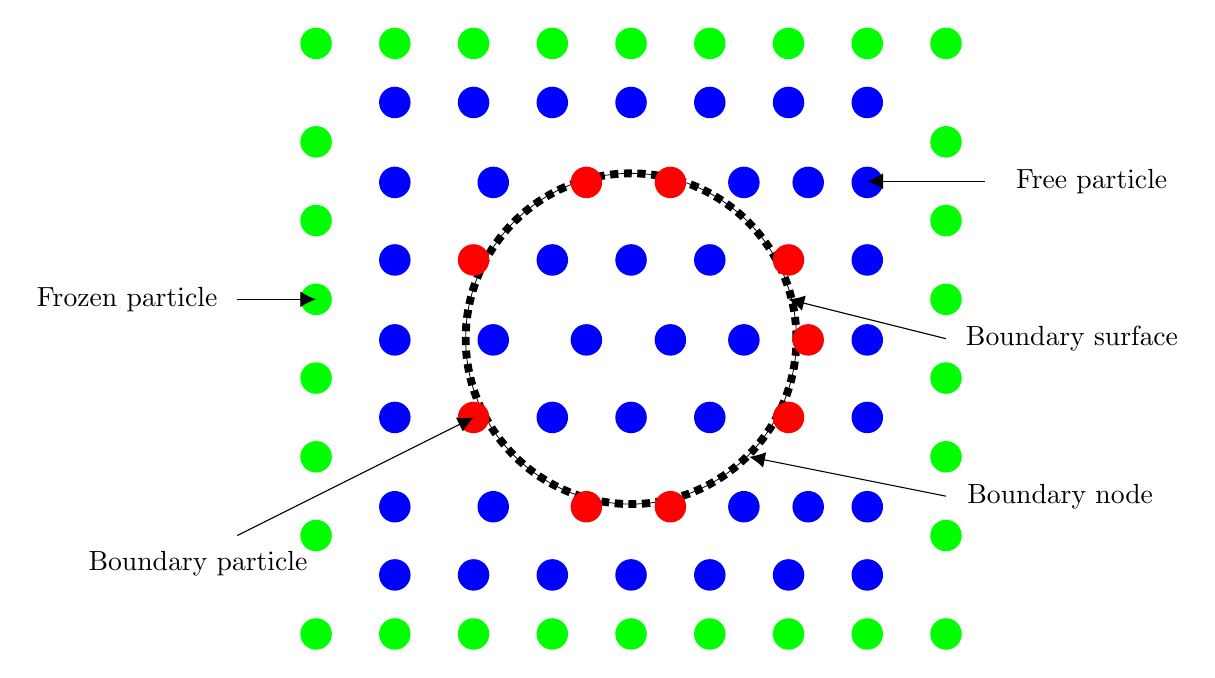
\begin{tikzpicture}
    \draw[line width=0.1mm](0,0) ellipse (2.1cm and 2.1cm);
    \draw[line width=1mm, dash dot](0,0) ellipse (2.1cm and 2.1cm);
    \foreach \x in {0,...,6}
        \foreach \y in  {0,...,3}
            {
              \pgfmathsetmacro{\xc}{\x - 3 * cos(\x / 10)};
              \pgfmathsetmacro{\yc}{2*(\y - 1.5 * cos(\y/10))};
              % Check if numbers are inside circle
              \pgfmathparse{ifthenelse(abs((\xc)^2 + (\yc)^2 - 2.1^2) <= 1.0,%
                  "red",
                  "blue")}
              \fill[\pgfmathresult] (\xc,\yc) circle (0.2);
    };
    \foreach \x in {0,...,6}
        \foreach \y in  {0,...,2}
            {
              \pgfmathsetmacro{\xc}{(\x - 3.0) + 0.5 * cos((\x-3.0)*30)};
              \pgfmathsetmacro{\yc}{2*(\y - 1.5) + 1.0* cos((\y-1.5)*20)};
              % Check if numbers are inside circle
              \pgfmathsetmacro{\res}{ifthenelse(abs((\xc)^2 + (\yc)^2 - 2.1^2) <= 1.0,%
                  "red",
                  "blue")}
              \fill[\res] (\xc,\yc) circle (0.2);
    };
    % external boundary

    \foreach \x in {1,...,9}
        \foreach \y in  {0,5}
            {
              \pgfmathsetmacro{\xc}{\x - 5};
              \pgfmathsetmacro{\yc}{1.5*(\y - 2.5)};
              % Check if numbers are inside circle
              \fill[green] (\xc,\yc) circle (0.2);
    };
    \foreach \x in {1, 9}
        \foreach \y in  {0,...,5}
            {
              \pgfmathsetmacro{\xc}{(\x - 5.0)};
              \pgfmathsetmacro{\yc}{(\y - 2.5)};
              % Check if numbers are inside circle
              \fill[green] (\xc,\yc) circle (0.2);
    };

    \draw[<-] (2.0,0.5) -- node[xshift=2.6cm, yshift=-0.25cm]{Boundary surface} (4,0.0);
    \draw[<-] (1.5,-1.5) -- node[xshift=2.7cm, yshift=-0.25cm]{Boundary node}(4, -2.);
    \draw[<-] (-2,-1.0) -- node[xshift=-2cm, yshift=-1.1cm]{Boundary particle}(-5,-2.5);
    \draw[<-] (3,2) -- node[xshift=2.1cm, yshift=0cm]{Free particle}(4.5,2);
    \draw[<-] (-4,0.5) -- node[xshift=-1.9cm, yshift=0cm]{Frozen particle}(-5,0.5);
  \end{tikzpicture}
  }
  \caption{Schematic of the initial distribution of particles and the
    different kinds of particles.}
  \label{fig:initial}
\end{figure}

The schematic shown in \cref{fig:initial} depicts the different kinds of
particles used in the proposed algorithm. In this figure, we consider the case
of a cylinder surrounded by fluid. The dashed black line represents the
surface of the cylinder (boundary surface), which we wish to capture
accurately. We assume that this surface is discretized into a set of points
called ``boundary nodes''. The different kinds of entities shown in the figure
are,
\begin{itemize}
\item \emph{Free particles}: These are particles arranged initially in a
  rectangular or hexagonal-packed pattern. Their motion is not constrained.
  These are depicted as blue circles.
\item \emph{Frozen particles}: These are a set of fixed dummy particles which
  surround the free particles in order to provide support to the kernel. These
  are depicted as green circles.
\item \emph{Boundary particles}: These particles are constrained to move along
  the ``boundary surface'' and are depicted as red circles.
\item \emph{Boundary surface}: The surface of the geometry that is
  discretized. It is represented by a set of fixed points, called ``boundary
  nodes'' which do not influence any other particles.
\item \emph{Boundary node}: These are points that discretize the boundary
  surface; they also store the local surface normals of the boundary surface.
  These are depicted as black dashes. We note that these are called nodes
  because they do not exert any forces on particles and only serve to provide
  information on the position and orientation of the boundary surface.
\end{itemize}
During the execution of the algorithm, free particles (blue) may be converted
to boundary particles (red) if they are close to the boundary surface. Once
the proposed algorithm completes, the red boundary particles must conform to
the boundary represented by the dashed black line. The blue particles inside
the dashed boundary will be considered as solid (dummy) particles and those
outside as fluid particles.

\begin{figure}[ht!]
  \centering
  \resizebox{10cm}{12cm}
  {
  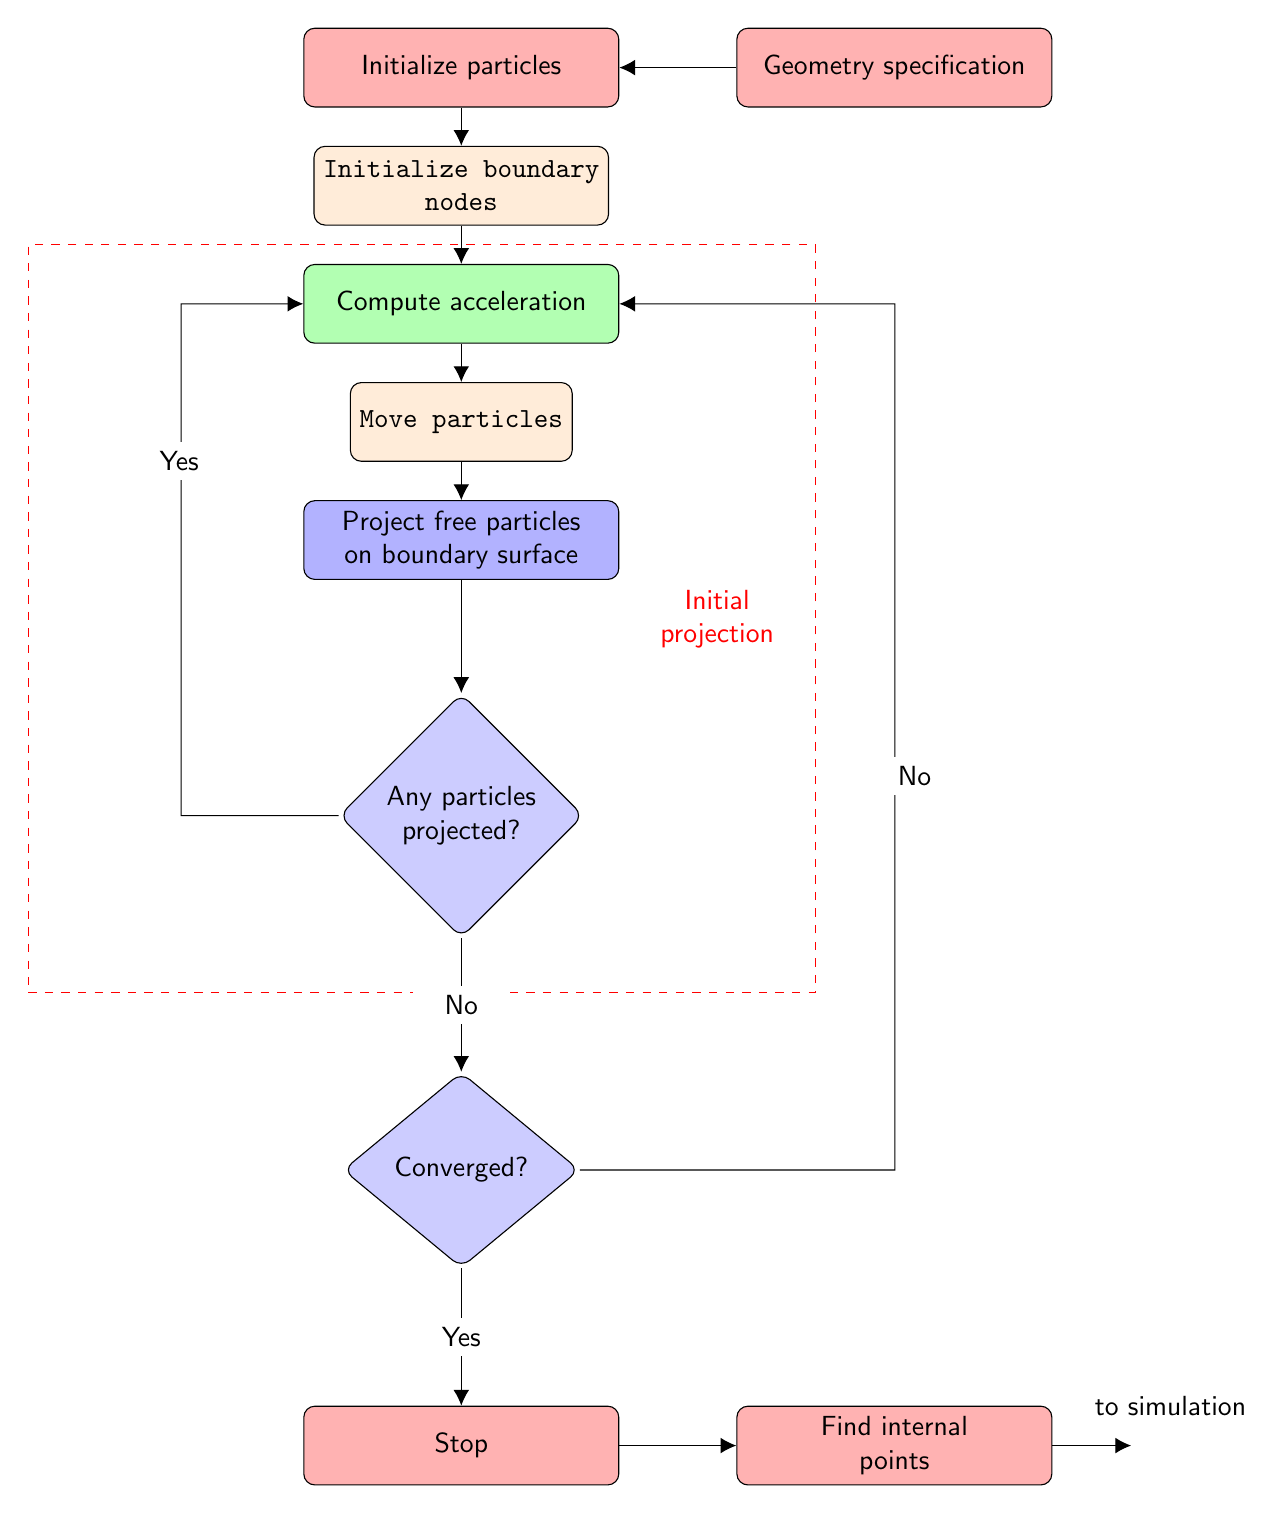
\begin{tikzpicture}[node distance=1.5cm,
    every node/.style={fill=white, font=\sffamily}, align=center]
  % Specification of nodes (position, etc.)
  \node [draw=red, dashed, shape=rectangle, minimum width=10cm, minimum height=9.5cm, anchor=center] at (-0.5,-7) {};
  \node(stage1)[text=red] at (3.25, -7) {Initial \\projection};
  \node (start) [startstop] {Initialize particles};
  \node (initialize) [process, below of=start] {Initialize boundary\\ nodes};
  \node (mesh) [startstop, right of=start, xshift=4cm] {Geometry specification};
  \node (compute) [activityRuns, below of=initialize] {Compute acceleration} ;
  \node (integrate) [process, below of=compute] {Move particles};
  \node (check) [activityStarts, below of=integrate] {Project free particles\\ on boundary surface};
  \node (projcheck) [decision, below of=check, yshift=-2cm]{Any particles\\ projected?};
  \node (convergence) [decision, below of=projcheck, yshift=-3cm] {Converged?};
  \node (stop) [startstop, below of=convergence, yshift=-2cm] {Stop};
  \node (internal) [startstop, right of=stop, xshift=4cm] {Find internal \\ points};

  % Specification of lines between nodes specified above
  % with aditional nodes for description
  \draw[->] (mesh) -- (start);
  \draw[->] (start) -- (initialize);
  \draw[->] (initialize) -- (compute);
  \draw[->] (compute) -- (integrate);
  \draw[->] (integrate) -- (check);
  \draw[->] (check) -- (projcheck);
  \draw[->] (projcheck) -- node[text width=1cm]{No}(convergence);
  \draw[->] (projcheck.west) -- ++(-2,0) -- ++(0,6.5) --
     node[xshift=-0.8cm,yshift=-2cm, text width=1cm]
     {Yes}(compute.west);
  \draw[->] (convergence) --  node[text width=1cm]{Yes}(stop);
  \draw[->] (convergence.east) -- ++(4,0) -- ++(0,11.0) --
     node[xshift=2.0cm, yshift=-6cm, text width=1cm]
     {No}(compute.east);
  \draw[->] (stop) --(internal);
  \draw[->] (internal.east) -- node[xshift=1cm, yshift=0.5cm]{to simulation}++(1.0,0);
  \end{tikzpicture}
}
  \caption{Flowchart of the particle packing algorithm.  The box outlined in
    dashed red lines is the initial projection phase.}
  \label{fig:flowchart}
\end{figure}

In \cref{fig:flowchart}, we show the overall flow of the algorithm. The
algorithm requires two inputs, the geometry information, and the desired
particle spacing. Given the geometry surface, we first estimate the number of
particles that should lie on this surface, $N_s$ using the desired spacing of
particles and the length of the surface in 2D (the surface area in 3D).

Initially, we create the frozen particles on the periphery of the domain placed on a rectangular lattice as shown in \cref{fig:initial}. Then, we place the free
particles inside the domain on a regular lattice. At this stage, we do not identify the boundary particles. We initialize the boundary nodes using the information provided by the user.

We compute the acceleration on the free particles and boundary particles (we
identify these later) using a local density gradient and a repulsive force.
The last step corresponds to the green block in \cref{fig:flowchart}. We move
the particles using the computed accelerations. As the free particles move, we
convert them to boundary particles if they are close enough to the boundary
surface. We project them to the nearest point on the boundary surface. The
boundary particles only move along the boundary surface. We convert the free
particles iteratively to boundary particles until no free particle is
sufficiently close to the boundary.

During the initial projection phase (denoted by the red dashed line in the
\cref{fig:flowchart}), we project the particles regularly onto the boundary
surface. We repeat the last step until the number of boundary particles has
reached $N_s$ and remains there for a few consecutive iterations. The
algorithm then proceeds to settle the particles into a uniform distribution
until the displacement of the particles is less than a user-defined
tolerance. We denote this step as the ``Converged'' block in
\cref{fig:flowchart}. Once we attain convergence, we obtain the boundary and
free particles packed inside and outside the surface as desired. Since the
boundary surface is known, we can quickly identify the free particles as solid
and fluid particles.

We can place this packed collection of free and boundary particles into a
larger regular mesh of particles for a simulation. For example, In
\cref{fig:sim} the dashed region shows where we can place the packed
particles. We use a regular mesh of the same spacing to represent the
exterior of this region (shown in green). This approach is convenient to use
in the context of fluid flow past solid bodies as done for internal
flows~\cite{negi2020improved} and free surface
flows~\cite{open_bc:tafuni:cmame:2018}. In the subsequent sections, we
explain the algorithm described above in detail.

\begin{figure}[ht!]
  \centering
  \resizebox{10cm}{7cm}{
  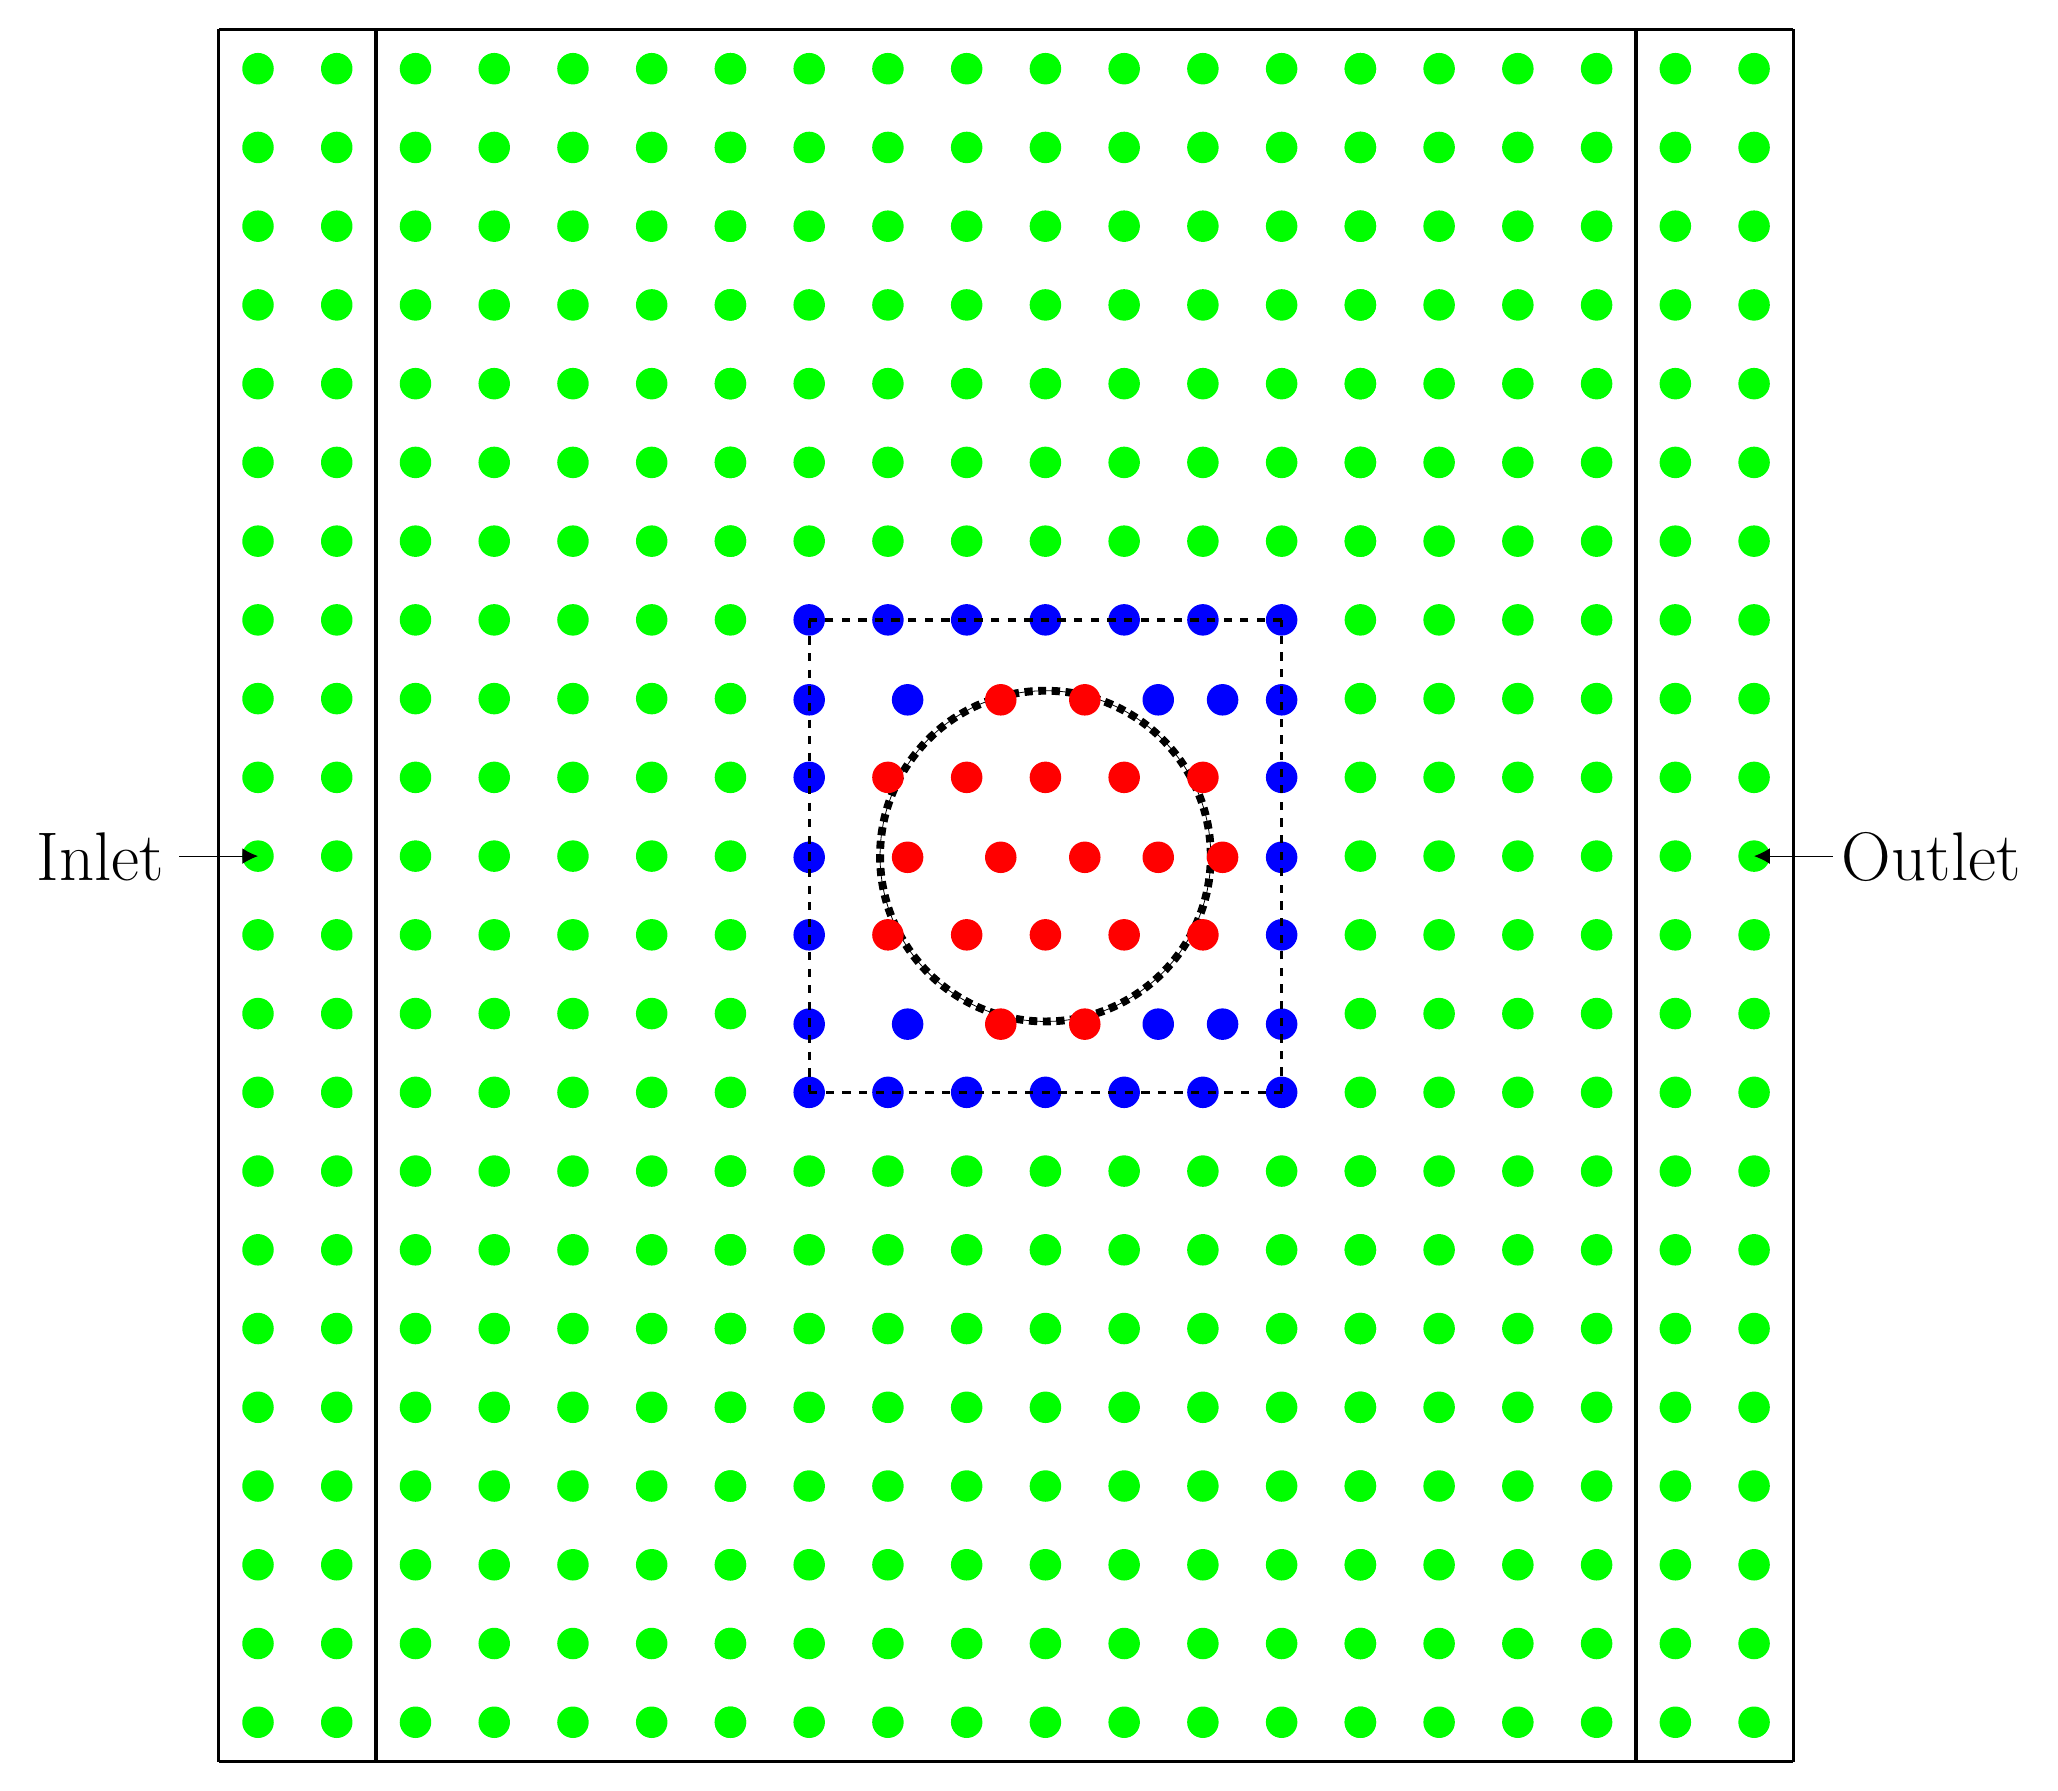
\begin{tikzpicture}
    \draw[line width=0.1mm](0,0) ellipse (2.1cm and 2.1cm);
    \draw[line width=1mm, dash dot](0,0) ellipse (2.1cm and 2.1cm);
    \foreach \x in {0,...,6}
        \foreach \y in  {0,...,3}
            {
              \pgfmathsetmacro{\xc}{\x - 3 * cos(\x / 10)};
              \pgfmathsetmacro{\yc}{2*(\y - 1.5 * cos(\y/10))};
              % Check if numbers are inside circle
              \pgfmathparse{ifthenelse((\xc)^2 + (\yc)^2 <= 2.4^2,%
                  "red",
                  "blue")}
              \fill[\pgfmathresult] (\xc,\yc) circle (0.2);
    };
    \foreach \x in {0,...,6}
        \foreach \y in  {0,...,2}
            {
              \pgfmathsetmacro{\xc}{(\x - 3.0) + 0.5 * cos((\x-3.0)*30)};
              \pgfmathsetmacro{\yc}{2*(\y - 1.5) + 1.0* cos((\y-1.5)*20)};
              % Check if numbers are inside circle
              \pgfmathsetmacro{\res}{ifthenelse((\xc)^2 + (\yc)^2 <= 2.4^2,%
                  "red",
                  "blue")}
              \fill[\res] (\xc,\yc) circle (0.2);
    };
    % external boundary

    \foreach \x in {1,...,9}
        \foreach \y in  {-7,...,0}
            {
              \pgfmathsetmacro{\xc}{\x - 5};
              \pgfmathsetmacro{\yc}{(\y - 4.0)};
              % Check if numbers are inside circle
              \fill[green] (\xc,\yc) circle (0.2);
    };
    \foreach \x in {1,...,9}
        \foreach \y in  {5,...,11}
            {
              \pgfmathsetmacro{\xc}{\x - 5};
              \pgfmathsetmacro{\yc}{(\y - 1.0)};
              % Check if numbers are inside circle
              \fill[green] (\xc,\yc) circle (0.2);
    };
    \foreach \x in {-5,...,1}
        \foreach \y in  {-10,...,11}
            {
              \pgfmathsetmacro{\xc}{(\x - 5.0)};
              \pgfmathsetmacro{\yc}{(\y - 1.0)};
              % Check if numbers are inside circle
              \fill[green] (\xc,\yc) circle (0.2);
    };
    \foreach \x in {9,...,14}
        \foreach \y in  {-10,...,11}
            {
              \pgfmathsetmacro{\xc}{(\x - 5.0)};
              \pgfmathsetmacro{\yc}{(\y - 1.0)};
              % Check if numbers are inside circle
              \fill[green] (\xc,\yc) circle (0.2);
    };

    % rectangle
    \draw[-, dashed, very thick] (-3, -3) -- (3, -3);
    \draw[-, dashed, very thick] (3, -3) -- (3, 3);
    \draw[-, dashed, very thick] (3, 3) -- (-3, 3);
    \draw[-, dashed, very thick] (-3, 3) -- (-3, -3);


    \draw[-, very thick] (-10.5, -11.5) -- (9.5, -11.5);
    \draw[-, very thick] (9.5, -11.5) -- (9.5, 10.5);
    \draw[-, very thick] (9.5, 10.5) -- (-10.5, 10.5);
    \draw[-, very thick] (-10.5, 10.5) -- (-10.5, -11.5);


    \draw[-, very thick] (-8.5, 10.5) -- (-8.5, -11.5);
    \draw[-, very thick] (7.5, 10.5) -- (7.5, -11.5);

    \draw [->] (-11, 0) -- node[xshift=-1.5cm]{\Huge Inlet} (-10, 0);
    \draw [->] (10, 0) -- node[xshift=1.75cm]{\Huge Outlet} (9, 0);

  \end{tikzpicture}
  }
	\caption{The pre-processed patch (dashed) of particles placed in the
    appropriate location of a typical simulation. The blue particles denote
    the free particles identified as fluid particles, and the red represents the
    solid particles identified by the packing process. The green particles are
    generated from a fixed mesh of points.}
	\label{fig:sim}
\end{figure}

\subsubsection{Initialization of boundary nodes}
\label{subsec:geom}

We first initialize the boundary nodes which represents the boundary surface.
In a two-dimensional domain, we require a set of points which discretize the
boundary curve. We parametrize the boundary curve by $\lambda$, and specify
the points on the curve as $\ten{x} = C(\lambda)$ and $ \lambda \in [0, 1]$.
We discretize this curve such that $\ten{x}_i = C(\lambda_i)$. We keep the
spacing between points such that $|\ten{x}_{i+1} - \ten{x}_i| < \Delta s$.
We initialize the boundary node coordinates using these points. We calculate
the outward normals $n_{x, i},n_{y, i}$ for any node $i$ using
\begin{equation}
  \begin{split}
  n_{x,i}  & =0.5  \left ( \frac{y_{i+1} - y_{i}}{d_{i+1, i}} +
   \frac{y_{i} - y_{i-1}}{d_{i, i-1}} \right) \\
  n_{y,i}  & =-0.5 \left( \frac{x_{i+1} - x_{i}}{d_{i+1, i}} +
  \frac{x_{i} - x_{i-1}}{d_{i, i-1}} \right)
  \end{split}
  \label{eq:2dnormal}
\end{equation}
where $d_{i, j}$ is the length of the segment joining the node at $(x_i, y_i)$
with the node at $(x_j, y_j)$. We normalize the resulting normal.
\Cref{eq:2dnormal} ensures that sharp corners of the curve have smooth
normals. For a three-dimensional case, a triangulation of the surface with
outward normals is necessary. One can generate the triangulation using any
mesh generation tool \cite{bern1992mesh}. We use the centroid of each triangle
and its normal to initialize the boundary nodes.

In SPH, the actual boundary surface is exactly in between the solid and fluid
particles. Thus, both in two and three dimensions, given a particle spacing of
$\Delta s$, we shift the boundary nodes by $\Delta s / 2$ inside the actual
boundary to correctly implement the solid boundary conditions as discussed in
\citet{marrone-deltasph:cmame:2011}. In order to move the nodes inwards, we
perform the following translation on each boundary node given by,
\begin{equation}
  \label{eq:trans}
  \ten{x} = \ten{x} - \frac{\Delta s}{2} \hat{\ten{n}},
\end{equation}
where, $\ten{x}$ is the position of the node and $\hat{\ten{n}}$ is its unit
normal pointing outwards. We must note that this is optional and one can
provide a pre-shifted surface and avoid the shifting with \cref{eq:trans}.

\begin{figure}[h!]
  \centering
  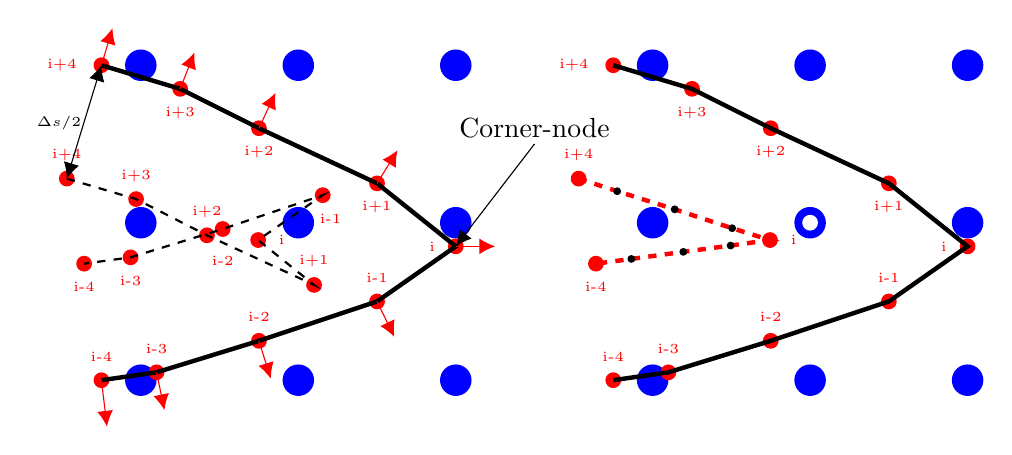
\begin{tikzpicture}
    \foreach \x in {2,...,4}
        \foreach \y in  {0,...,2}
            {
              \pgfmathsetmacro{\xc}{\x*2};
              \pgfmathsetmacro{\yc}{\y*2};
              % Check if numbers are inside circle
              \fill[blue] (\xc,\yc) circle (0.2);
    };

    \foreach \x in {2,...,4}
        \foreach \y in  {0,...,2}
            {
              \pgfmathsetmacro{\xc}{\x*2 + 6.5};
              \pgfmathsetmacro{\yc}{\y*2};
              % Check if numbers are inside circle
              \fill[blue] (\xc,\yc) circle (0.2);
    };

    \fill[red] (3.5, 4) circle(0.1) node[xshift=-0.5cm]{\tiny i+4};
    \fill[red] (4.5, 3.7) circle(0.1)node[yshift=-0.3cm]{\tiny i+3};
    \fill[red] (5.5, 3.2) circle(0.1)node[yshift=-0.3cm]{\tiny i+2};
    \fill[red] (7, 2.5) circle(0.1)node[yshift=-0.3cm]{\tiny i+1};
    \fill[red] (8, 1.7) circle(0.1)node[xshift=-0.3cm]{\tiny i};
    \fill[red] (7, 1.) circle(0.1)node[yshift=0.3cm]{\tiny i-1};
    \fill[red] (5.5, 0.5) circle(0.1)node[yshift=0.3cm]{\tiny i-2};
    \fill[red] (4.2, 0.1) circle(0.1)node[yshift=0.3cm]{\tiny i-3};
    \fill[red] (3.5, 0) circle(0.1)node[yshift=0.3cm]{\tiny i-4};

    \draw[-, ultra thick] (3.5, 4) -- (4.5, 3.7) --(5.5, 3.2)-- (7, 2.5) -- (8, 1.7) -- (7, 1.) -- (5.5, 0.5) -- (4.2, 0.1)-- (3.5, 0);

    \fill[red] (3.5+6.5, 4) circle(0.1) node[xshift=-0.5cm]{\tiny i+4};
    \fill[red] (4.5+6.5, 3.7) circle(0.1)node[yshift=-0.3cm]{\tiny i+3};
    \fill[red] (5.5+6.5, 3.2) circle(0.1)node[yshift=-0.3cm]{\tiny i+2};
    \fill[red] (7+6.5, 2.5) circle(0.1)node[yshift=-0.3cm]{\tiny i+1};
    \fill[red] (8+6.5, 1.7) circle(0.1)node[xshift=-0.3cm]{\tiny i};
    \fill[red] (7+6.5, 1.) circle(0.1)node[yshift=0.3cm]{\tiny i-1};
    \fill[red] (5.5+6.5, 0.5) circle(0.1)node[yshift=0.3cm]{\tiny i-2};
    \fill[red] (4.2+6.5, 0.1) circle(0.1)node[yshift=0.3cm]{\tiny i-3};
    \fill[red] (3.5+6.5, 0) circle(0.1)node[yshift=0.3cm]{\tiny i-4};

    \draw[-, ultra thick] (3.5+6.5, 4) -- (4.5+6.5, 3.7) --(5.5+6.5, 3.2)-- (7+6.5, 2.5) -- (8+6.5, 1.7) -- (7+6.5, 1.) -- (5.5+6.5, 0.5) -- (4.2+6.5, 0.1)-- (3.5+6.5, 0);

    \draw[red, ->] (3.5, 4) -- (3.64, 4.47);
    \draw[red, ->] (4.5, 3.7) -- (4.68, 4.16);
    \draw[red, ->] (5.5, 3.2) -- (5.71, 3.65);
    \draw[red, ->] (7, 2.5) -- (7.26, 2.92);
    \draw[red, ->] (8, 1.7) -- (8.5, 1.7);
    \draw[red, ->] (7, 1.) -- (7.22, 0.55);
    \draw[red, ->] (5.5, 0.5) -- (5.65, 0.02);
    \draw[red, ->] (4.2, 0.1) -- (4.30, -0.38);
    \draw[red, ->] (3.5, 0) -- (3.57, -0.59);

    \fill[red] (3.06, 2.56) circle(0.1) node[yshift=0.3cm] {\tiny i+4};
    \fill[red] (3.94, 2.30) circle(0.1) node[yshift=0.3cm] {\tiny i+3};
    \fill[red] (4.84, 1.84) circle(0.1) node[yshift=0.3cm] {\tiny i+2};
    \fill[red] (6.20, 1.21) circle(0.1) node[yshift=0.3cm] {\tiny i+1};
    \fill[red] (5.49, 1.78) circle(0.1) node[xshift=0.3cm] {\tiny i};
    \fill[red] (6.31, 2.35) circle(0.1) node[yshift=-0.3cm, xshift=0.1cm] {\tiny i-1};
    \fill[red] (5.04, 1.92) circle(0.1) node[yshift=-0.4cm] {\tiny i-2};
    \fill[red] (3.87, 1.56) circle(0.1) node[yshift=-0.3cm] {\tiny i-3};
    \fill[red] (3.28, 1.48) circle(0.1) node[yshift=-0.3cm] {\tiny i-4};

    \draw[dashed, -, thick](3.06, 2.56) -- (3.94, 2.30) -- (4.84, 1.84) --
    (6.20, 1.21) -- (5.49, 1.78) -- (6.31, 2.35) -- (5.04, 1.92) -- (3.87,
    1.56) -- (3.28, 1.48);


    \draw[red, -, dashed, ultra thick](3.06+6.5,2.56) -- (3.55+6.5,2.40) --
    (4.28+6.5,2.17) -- (5.01+6.5,1.93) -- (5.49+6.5,1.78) -- (4.99+6.5,1.71)
    -- (4.39+6.5,1.63) -- (3.73+6.5,1.54) -- (3.28+6.5,1.48);

    \fill[red] (3.06+6.5, 2.56) circle(0.1) node[yshift=0.3cm] {\tiny i+4};
    \fill[black] (3.55+6.5,2.40) circle(0.05);
    \fill[black] (4.28+6.5,2.17) circle(0.05);
    \fill[black] (5.01+6.5,1.93) circle(0.05);
    \fill[red] (5.49+6.5, 1.78) circle(0.1) node[xshift=0.3cm] {\tiny i};
    \fill[black] (4.99+6.5,1.71) circle(0.05);
    \fill[black] (4.39+6.5,1.63) circle(0.05);
    \fill[black] (3.73+6.5,1.54) circle(0.05);
    \fill[red] (3.28+6.5, 1.48) circle(0.1) node[yshift=-0.3cm] {\tiny i-4};


    \draw[<-] (8, 1.7) -- (9, 3.0) node[yshift=0.2cm]{Corner-node};
    \draw[<->] (3.5, 4) -- (3.06, 2.56) node[yshift=0.7cm, xshift=-0.1cm]{\tiny $\Delta s/2$};
    \fill[white] (6+6.5,2) circle (0.1);
\end{tikzpicture}
\caption{Shifting of the boundary near a sharp edged boundary. The boundary
  nodes are depicted in red with normals. On the left is the boundary surface
  after the initial shifting shown as black dashed lines. On the right is the
  final geometry after removal of the intersecting edges which are shown as
  dashed red lines. The annular blue free particle is the candidate to be
  placed on the corner and held fixed.}
	\label{fig:corner_node}
\end{figure}


One must take care when there are sharp changes in the features of the
geometry. Consider an airfoil trailing edge in \cref{fig:corner_node} shown
as a black line. We mark the sharp corners as ``corner nodes'', and in this
case it is the $i$\textsuperscript{th} node. When we shift the nodes on this
surface, the boundary surface tends to self-intersect itself. This is shown
by the red nodes connected using a black dashed line. In order to remove the
intersection of the boundary surface near the corner node, we replace the
points $i-3$ to $i-1$ by the points on the line joining $i-4$ and $i$ with
equal spacing shown by black points. Similarly we also replace the points
$i+1$ to $i+3$ with points lying along the line joining points $i$ and $i+4$.
This results in a non-intersecting surface, as shown by the red dashed line
on the right side of \cref{fig:corner_node}. Once we resolve the
intersection, we place the nearest free particle near the corner node
(annular blue particle) on it and convert it to a \emph{fixed boundary
particle}. The position of these fixed boundary particles does not change in
the entire simulation.

In the case of a three-dimensional object, one has to make sure that the
surface does not intersect after applying \cref{eq:trans} or use a pre-shifted
surface as an input.


\subsubsection{Dynamics of the particles}
\label{subsec:pm}

In this section, we discuss the dynamics of particle regularization.
We apply two forces to the particles, and together these regularize the
particle distribution. The two forces are a gradient due to particle
disorder and a pure inter-particle repulsive force.

In the presence of a constant pressure field, $p_b$ and no viscous effect, the
momentum equation (\cref{eq:mom}), becomes
\begin{equation}
  \label{eq:backgrounpressure}
  \frac{d \ten{u}}{dt} = -\frac{\nabla (1 \cdot p_b)}{\rho} =
  -\frac{p_b \nabla(1) + \nabla(p_b)}{\rho}.
\end{equation}

When the term, $p_b \nabla(1)$, on the right hand side is discretized using
the SPH method, we obtain $p_b \nabla \Gamma$ (see \cref{eq:del-gamma}). This
is non-zero when the particles are not uniform and hence particles exert a
force on each other in order to reach an equilibrium position. Using the SPH
approximation, we discretize the above equation as
\begin{equation}
  \label{eq:backgrounpressure_sph}
  \ten{a}_{b,i} = \frac{d \ten{u}_i}{dt} =
  - p_b \sum_j \frac{V_i V_j}{m_i}\nabla W_{ij},
\end{equation}
where $V_i = \frac{m_i}{\rho_i}$ is the volume of the $i$\textsuperscript{th}
particle, $\rho_i$ is the density, $W_{ij}$ is the kernel function chosen for
the SPH discretization. The summation is over all the neighbors of
$i^\text{th}$ particle. Since all SPH kernels satisfy \cref{eq:cond}, any
suitable SPH kernel discussed in \cref{sec:sph} can be employed. In this
paper, the quintic spline kernel is used given by,
\begin{equation}
	\label{eq:quintic-spline}
	W(q) = \left \{
	\begin{array}{ll}
		\sigma \left[ {(3-q)}^5 - 6{(2-q)}^5 + 15{(1-q)}^5 \right] \
		& \textrm{for} \ 0\leq q \leq 1,\\
		\sigma \left[ {(3-q)}^5 - 6{(2-q)}^5 \right]
		& \textrm{for} \ 1 < q \leq 2,\\
		\sigma \ {(3-q)}^5  & \textrm{for} \ 2 < q \leq 3,\\
		0 & \textrm{for} \ q>3,\\
	\end{array} \right.
\end{equation}
where, $\sigma = 1/(120 h), 7/(478\pi h^2),1/(120\pi h^3) $ in one, two and
three-dimensions respectively and $q=|\ten{r}|/h$. In this algorithm, the
value of $p_b$ is set to $1$ independent of the resolution. In addition to
this force, we use a repulsive force (RF) similar to the gradient of the
Lennard Jones potential (LJP). The new repulsion force potential
($\phi_{RF}$) is given by
\begin{equation}
  \label{eq:LJP}
  \phi_{RF} = 12 \ k_r \left( \frac{c^2}{r^3} - \frac{c}{r^2} \right)\\
\end{equation}
where $k_r$ is a constant. We set $c = 2 \alpha \Delta s/3 $, where $\alpha$
is a scaling factor. The gradient of \cref{eq:LJP} gives us the force due to
$\phi_{RF}$.  We keep the force constant for $r<\Delta s / 2$ in order to avoid
very large repulsion forces. We write the SPH approximation of the acceleration due to \cref{eq:LJP} as
\begin{equation}
  \label{eq:LJPacc_sph}
  \ten{a}_{RF,i} = -\nabla \phi_{RF,i} =
  \left \{
    \begin{array}{ll}
    \sum_j 192 \ k_r \ten{e}_{ij}
    \left( \frac{3  c^2}{\Delta s^4} - \frac{c}{\Delta s^3} \right)& r_{ij} \leq \Delta s/2\\
    \sum_j 12 \ k_r \ten{e}_{ij}
    \left( \frac{3c^2}{r_{ij}^4} - \frac{2c}{r_{ij}^3} \right)
    & \Delta s/2 < r_{ij} \leq \alpha \Delta s \\
    0 & r_{ij} >  \alpha \Delta s\\
    \end{array} \right.
\end{equation}
where $\ten{e}_{ij} = \ten{x}_{ij}/r_{ij}$. Note that the acceleration is
continuous at $r_{ij} = \Delta s/2$. We find that using a value of
$\alpha=0.95$ works well for the algorithm.

It is clear from \cref{eq:LJPacc_sph} that this force is active only when
particles come closer than the desired particle spacing. This force prevents
particle pairing, which may happen due to the use of some kernels like cubic
spline for large time steps \cite{dehnen-aly-paring-instability-mnras-2012}.
In \cref{fig:ljp}, we show the comparison between the force due to LJP and RF. The LJP repulsion force increases rapidly compared to our suggested
repulsion force. Thus, This force allows us to use a larger time step during integration.
Moreover, unlike the force due to LJP, the new force does not introduce
inter-particle attraction.
\begin{figure}[ht!]
  \centering
  \ifthenelse{\showimages=1}
  {
    \includegraphics[width=\textwidth]{figures/force/force.png}
  }{}
  \caption{Force due to LJ potential and the gradient of \cref{eq:LJP} as a
    function of distance, $r$ and $\alpha=1$.}
  \label{fig:ljp}
\end{figure}

As discussed in~\cite{colagrossi2012particle}, for stability, we use a
damping force to reduce the energy of the system. We compute the acceleration
due to damping for the $i^\text{th}$ particle by
\begin{equation}
  \label{eq:damp_sph}
 \ten{a}_{d,i} = -\zeta \ten{u}_i
\end{equation}
where $\zeta$ is the damping constant and $\ten{u}_i$ is the velocity of the
$i^\text{th}$ particle. We discuss the value of the damping constant $\zeta$ in \cref{subsec:time}. Thus, the equation governing the dynamics of
the system is
\begin{equation}
  \label{eq:total_force}
  \begin{split}
 \frac{du}{dt} &= -\frac{\nabla p_b}{\rho} - \nabla \phi_{RF} - \zeta \ten{u}.\\
  \end{split}
\end{equation}
We convert the above equation into SPH form using
\cref{eq:backgrounpressure_sph,eq:LJPacc_sph,eq:damp_sph}; thus acceleration
of the $i^\text{th}$ particle,
\begin{equation}
  \label{eq:total_force_i}
  \begin{split}
  \ten{a}_i &= \ten{a}_{b,i} + \ten{a}_{RF,i} + \ten{a}_{d,i}. \\
  \end{split}
\end{equation}
We must note that the combination of background pressure and
repulsion forces produces repulsion only when particles are disordered. One
can also accomplish this by using the particle shifting techniques (PST)
first proposed by \cite{xu2009accuracy}.

On using \cref{eq:total_force}, we calculate the velocities and new positions
using a semi-implicit Euler integration given by,
\begin{equation}
  \label{eq:velocity}
  \begin{split}
 \ten{u}_i(t + \Delta t) &= \ten{u}_i(t) + \Delta t \ten{a}_{i}(t) \\
 \ten{x}_i(t + \Delta t) &= \ten{x}_i(t) + \Delta t \ \ten{u}_i(t+\Delta t)
\end{split}
\end{equation}
In the case of boundary particles, we correct the velocities to constrain
them to move along the surface (discussed in \cref{subsec:om}). We should
note that the packing algorithm only ensures that particle distributions are
regular and therefore using a higher-order integrator would not promise
better results.

We study the stability of the method in a two and three-dimensional domain
for finite perturbation under the action of forces described above. We
consider a domain of size 1 unit along each coordinate direction. We place
particles with a spacing of $\Delta s = 0.05$. We also place fixed particles
outside this unit box suitably. The value of $p_{b}$, $\zeta$, $k_r$ and
$\Delta t$ are set as discussed in \cref{subsec:time}. We perturb a single
particle close to the center by $\Delta s / 2$ in each direction. We move the
particles using \cref{eq:total_force} and \cref{eq:velocity} for 15000
iterations. We consider the stability of the following initial distribution
of particles:

\begin{figure}[ht!]
  \begin{subfigure}{0.5\textwidth}
    \centering
    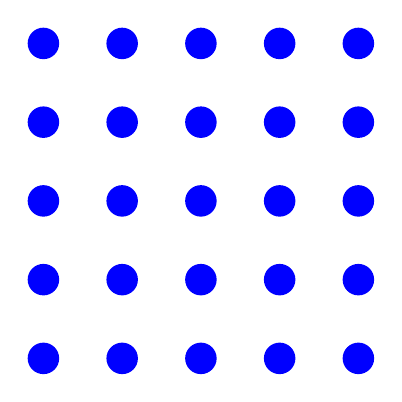
\begin{tikzpicture}
      \foreach \x in {0,...,4}
          \foreach \y in  {0,...,4}
              {
                \pgfmathsetmacro{\xc}{\x};
                \pgfmathsetmacro{\yc}{\y};
                % Check if numbers are inside circle
                \fill[blue] (\xc,\yc) circle (0.2);
      };
    \end{tikzpicture}
    \caption{Rectangular}
    \label{fig:rect}
  \end{subfigure}
  \begin{subfigure}{0.5\textwidth}
    \centering
    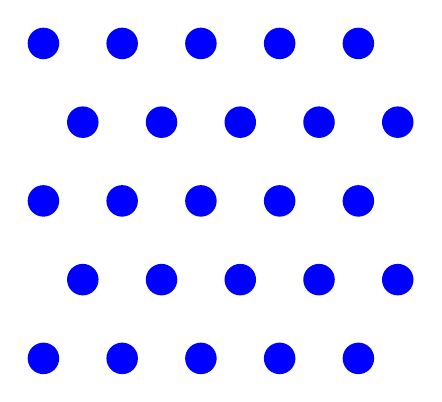
\begin{tikzpicture}
      \foreach \x in {0,...,4}
          \foreach \y in  {0,...,2}
              {
                \pgfmathsetmacro{\xc}{\x};
                \pgfmathsetmacro{\yc}{\y*2.};
                % Check if numbers are inside circle
                \fill[blue] (\xc,\yc) circle (0.2);
      };
      \foreach \x in {0,...,4}
          \foreach \y in  {0,...,1}
              {
                \pgfmathsetmacro{\xc}{\x*1.+0.5};
                \pgfmathsetmacro{\yc}{\y*2.+1};
                % Check if numbers are inside circle
                \fill[blue] (\xc,\yc) circle (0.2);
      };
    \end{tikzpicture}
    \caption{Hexagonal}
    \label{fig:hex}
  \end{subfigure}
  \caption{Different packing structures in 2D.}
  \label{fig:packing}
\end{figure}

\begin{itemize}
  \item hexagonal packing shown in \cref{fig:hex} with number density ($ND$) gradient.
  \item hexagonal packing shown in \cref{fig:hex} with $ND$ + repulsion force ($RF$).
  \item rectangular packing shown in \cref{fig:rect} with $ND$ gradient.
  \item rectangular packing shown in \cref{fig:rect} with $ND + RF$.
\end{itemize}

We evaluate the error in every iteration using
\begin{equation}
  L_{\infty}(\rho - \rho_{o}) = \max(\{(\rho_i - \rho_{o}) ,  \forall i \in 1..N \})
\end{equation}
where $N$ is the number of particles in the domain. In \cref{fig:2d1} and
\cref{fig:3d1}, we plot the $L_{\infty}(\rho - \rho_{o})$ with number of
iterations for 2D and 3D domain respectively with $\rho_{o}=1.0$. In 2D, all
the combinations perform well. In the case of the 3D domain, rectangular
lattices settle into an equilibrium configuration with a much larger density
difference. Therefore the rectangular lattice in 3D is an unstable
equilibrium. In contrast, the hexagonal packing in 3D is in a stable
equilibrium.

We can understand the behavior in 3D from the total potential energy of the
particles. We can see that \cref{eq:gamma} for $\Gamma_i$ is the potential
energy of the $i$\textsuperscript{th} particle and hence $\sum_i \Gamma_i $
is the total potential energy of the system. The acceleration of a particle
given in \cref{eq:backgrounpressure} is the negative of the gradient of its
potential energy. We have numerically found that a small perturbation of a
particle at a given site reduces the total potential energy in the rectangular lattice case, whereas the same perturbation results in higher
potential energy in the case of the hexagonal packing. It suggests that the
hexagonal packing is stable in 3D, unlike the rectangular lattice. A careful
analysis of the stability is outside the scope of the present work. Due to
the stability of hexagonal packing shown in \cref{fig:hex}, we use it in all
our test cases.

\begin{figure}[ht!]
  \begin{subfigure}{0.5\textwidth}
    \centering
    \ifthenelse{\showimages=1}
    {
    \includegraphics[width=\textwidth]{figures/stability_2d/stability_2d_perturbed.png}
    }{}
    \caption{2D}
    \label{fig:2d1}
  \end{subfigure}
  \begin{subfigure}{0.5\textwidth}
    \centering
    \ifthenelse{\showimages=1}
    {
    \includegraphics[width=\textwidth]{figures/stability_3d/stability_3d_perturbed.png}
    }{}
    \caption{3D}
    \label{fig:3d1}
  \end{subfigure}
  \caption{Density convergence with a particle at center perturbed by $\Delta
  s/4$.}
  \label{fig:pert}
\end{figure}


\subsubsection{Projecting free particles to the surface}
\label{subsec:pa_add}

Initially, the boundary particles are unlikely to conform to the boundary
surface. At $t=0$, we assign no particles as boundary particles. We convert
free particles to boundary particles after every $50$ iteration. We refer to
this as the ``projection frequency''. The projection frequency is a user-defined
parameter. Increasing this does not guarantee better results; however, we do
not recommend a very small value. On running the proposed algorithm with
spacing $\Delta s = 0.1$ around a unit radius 2D cylinder with varying
projection frequency as shown in \cref{fig:dfreq}, we found that after
projection frequency $20$, the number density gradient does not change by a
large value. Thus, we choose the value $50$ heuristically.

\begin{figure}
  \centering
  \includegraphics[width=0.8\textwidth]{figures/pfreq_test/pfreq_test_fig}
  \caption{Error in $\nabla \Gamma_i$ for domain with unit radius cylinder with different projection frequency.}
  \label{fig:dfreq}
\end{figure}


\begin{algorithm}[h!]
  \SetAlgoLined
  \KwIn{\lstinline{proj_freq, ds=}$\Delta s$}
  \KwResult{List of free particles to be projected}
  \code{iteration} = 0\;
  \lstinline{empty_count} = 0\;
  \While{\codek{not converged}} {
    \ldots\;
    \If{\codek{iteration \% proj_freq == 0}}{
      \eIf{ \lstinline{empty_count < 4}} {
        \lstinline{p_list = FindParticlesNearBoundary}(\code{maxdist=0.5*ds)}\;
        \eIf {\codek{len(p_list) > 0}}{
          \code{ConvertParticles()}\;
          \lstinline{empty_count} = 0\;
        }{
          \lstinline{empty_count}++\;
        }

      } {
        \lstinline{p_list = FindParticlesNearBoundary(maxdist=0.65*ds)}\;
        \code{ConvertParticles()}\;
      }
      \code{ProjectToBoundary()}\;
      \ldots\;
    }
    \code{iteration++}\;
  }
  \caption{Pseudo-code for free particle projection.}
  \label{alg:proj}
\end{algorithm}

If we consider a flat surface, an estimate for the number of particles that
can fill the surface is, $N_s= A_s/\Delta s^{(d-1)}$ where $A_s$ is the area
of the surface and $d$ is the dimension of the space in which the surface is
embedded. In order to perform projection, we employ two different criteria
depending upon whether the initial projection in \cref{fig:flowchart} is
complete or not, as shown in algorithm \ref{alg:proj}.

\begin{sloppypar}
In the algorithm, the function \lstinline{FindParticlesNearBoundary} finds
all the free particles that are less than a prescribed distance,
\lstinline{maxdist}, to a boundary node. We compute the distance as follows,
given a free particle $p$, we find the boundary node $b$ that is closest and
compute the distance $\ten{r}_{pb} \cdot \ten{n}_b$, where $\ten{r_{pb}} =
\ten{r}_p - \ten{r}_b$ and $\ten{n}_b$ is the normal at $b$. We note that the
algorithm to find the nearest boundary node uses the existing neighbors
generated when computing the accelerations discussed in \cref{subsec:pm}.
\end{sloppypar}

\begin{sloppypar}
The \lstinline{empty_count} variable stores the number of consecutive passes
for which the \lstinline{p_list} was empty. We convert the free particles
having a distance to the boundary node less than $0.5 \Delta s$ to boundary
particles in \code{ConvertParticles} and project them to the boundary surface
in \code{ProjectToBoundary}. However, if the \lstinline{empty_count} exceeds
3, we increase the distance threshold to $0.65 \Delta s$. We increase the
threshold to handle the corner cases where free particles are just outside
$0.5 \Delta s$ distance\footnote{We find this value based on numerical
experiments. Too small a value like $0.55 \Delta s$ produces poor results in
coarse resolutions, and too large a value ($0.75 \Delta s$) produced poor
distributions with finer resolutions.}. This iterative conversion of free
particles to boundary particles is necessary in order to capture the surface
accurately.
\end{sloppypar}

\subsubsection{Kinematics of boundary particles}
\label{subsec:om}

\begin{figure}[ht!]
  \centering

  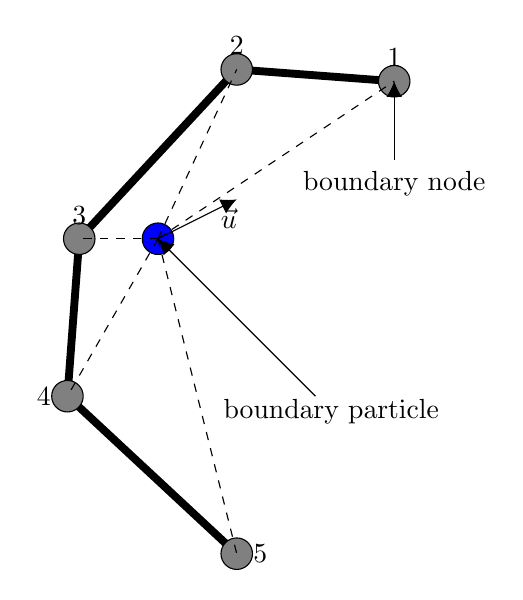
\begin{tikzpicture}

    \draw [-, line width=1mm] (2,-4) -- (-0.15,-2)-- (0, 0) -- (2,2.15) -- (4, 2);
    \draw[fill=gray](0,0) ellipse (2mm and 2mm) node[yshift=3mm]{3};
    \draw[fill=gray](2,-4) ellipse (2mm and 2mm) node[xshift=3mm]{5};
    \draw[fill=gray](4,2) ellipse (2mm and 2mm) node[yshift=3mm]{1};
    \draw[fill=gray](-0.15,-2) ellipse (2mm and 2mm) node[xshift=-3mm]{4};
    \draw[fill=gray](2,2.15) ellipse (2mm and 2mm) node[yshift=3mm]{2};

    \draw[fill=blue] (1,0) ellipse (2mm and 2mm);
    \draw[->] (1,0) -- node[xshift=0.4cm]{$\vec{u}$}(2,0.5);

    \draw[-, dashed] (1,0) -- (2,-4);
    \draw[-, dashed] (1,0) -- (-0.15,-2);
    \draw[-, dashed] (1,0) -- (0,0);
    \draw[-, dashed] (1,0) -- (2,2.15);
    \draw[-, dashed] (1,0) -- (4,2);

    \draw[<-] (1,0) -- node[xshift=1.2cm, yshift=-1.2cm]{boundary particle}(3,-2);
    \draw[<-] (4,2) -- node[yshift=-0.8cm]{boundary node}(4, 1);

    \end{tikzpicture}
  \caption{Motion of boundary particle along the geometry.}
  \label{fig:bm}
\end{figure}

As discussed earlier, we constrain the movement of the boundary particles
along the boundary surface. \Cref{fig:bm} illustrates the motion of nodes 1,
2, 3, 4, and 5 representing boundary particles (in blue) moving along the
geometry. We note that even though the particle is a boundary particle, it is
only projected onto the surface every \lstinline{proj_freq} time steps as
discussed in \cref{subsec:pa_add} hence the boundary particle may not exactly
lie on the boundary as it moves.

We perform the motion of the boundary particle as follows. We first identify
the boundary node nearest to the boundary particles in the direction of the
particle's velocity. Consider a boundary particle $p$, and a boundary node
$j$, near $p$ having position $\ten{x}_{p}$ and $\ten{x}_j$ respectively. We
determine the index of the nearest node, $J$ by
\begin{equation}
  \label{eq:dir}
  J = \argmin_j \{r_{pj}\ |\ j \in \mathcal{N}_{p}\ \text{and} \
    \ten{x}_{pj} \cdot \ten{u}_{p} < 0\}
\end{equation}
where, $\ten{x}_{pj} = \ten{x}_p - \ten{x}_j$, $r_{pj} = |\ten{x}_{pj}|$,
$\ten{u}_p$ is the velocity of the boundary particle and $\mathcal{N}_p$ is
the set of neighboring nodes of $p$. In \cref{fig:bm}, the node $2$ satisfies
the conditions in \cref{eq:dir}, and so $J=2$. Using the nearest node index
$J$, and the boundary particle $p$, the direction of motion $\hat{\ten{x}}_r
= -\hat{\ten{x}}_{pJ}$ (where $\hat{\ten{x}} = \ten{x}/|\ten{x}|$). Thus, we
update the boundary particle position using the following equation
\begin{equation}
  \label{eq:int_solid}
  \ten{x}_{p}^{m+1} = \ten{x}_{p}^m +  (\ten{u}_{p}^{m+1} \cdot \hat{\ten{x}}^m_{r})\hat{\ten{x}}^m_{r} \Delta t,
\end{equation}
where $m$ is the time step.

\subsubsection{Convergence criteria} \label{subsec:conv}

For a perfectly packed distribution of particles, each particle should satisfy
the second condition in \cref{eq:cond1} i.e.\ $\nabla \rho_i = 0$.
However, this would take a lot of computational time. In case of geometries
having irrational volumes like the unit circle (V=$\pi$), one could never
achieve a perfect convergence, given a fixed resolution. Thus, similar to
\cite{jiang2015blue}, we use the following criteria for convergence,
\begin{equation}
  \label{eq:conv}
  \frac{\max(u_{i}) \Delta t}{h} < \epsilon
\end{equation}
where, $\epsilon=10^{-4}$ is the tolerance for all our test cases, $u_{i}$ is
the velocity magnitude of $i$\textsuperscript{th} particle, and we take the maximum over all the particles.


\subsubsection{Determining the constants and time-step}
\label{subsec:time}

It is important to choose the parameters $\zeta$ and $k_r$ appropriately. We
observe that the \cref{eq:backgrounpressure_sph} scales as $O(p_b \Delta
s^{-1})$ and \cref{eq:LJPacc_sph} scales as $O(k_r \Delta s^{-2})$. By
requiring that these forces be of the same order, we can derive the relation
\begin{equation}
  \frac{k_r}{p_b} = C \Delta s
\end{equation}
where C is an arbitrary constant. To find a suitable value, we consider a 2D
lattice of points. We then perturb a single particle by $\Delta s/4$ in each
direction. We apply a similar procedure to a 3D lattice. We find that a value
of $C$ in the range $0.004 - 0.006$ ensures that the two forces are of the
same order.

In order to ensure stability, the damping constant has a form similar to the
one suggested by \citet{colagrossi2012particle} given by $\zeta =
C_{\zeta}/\Delta s$, where $C_{\zeta}$ is set in the range $0.2-0.5$
resulting in an underdamped system.

The time step, $\Delta t$ is set as in \citet{Adami2013} given by,
\begin{equation}
  \begin{split}
    \Delta t_{p_b} &= 0.1 \frac{h}{p_b} \\
    \Delta t_{\zeta} &= \sqrt{0.1 \frac{h}{\zeta u_{i}}} \\
    \Delta t &= \min(\Delta t_{p_b}, \Delta t_{\zeta})\\
  \end{split}
\end{equation}
where $u_i$ is the velocity magnitude of the $i^{th}$ particle. We note that
we have used a $p_b=1$ for all our simulations.

\subsubsection{Separating interior and exterior particles}
\label{subsec:inter}

At the end of the simulation, we obtain interior (particles inside the
boundary surface) and exterior particles (particles outside the boundary
surface) uniformly distributed. We extract and use the interior particles and the boundary particles as solid particles, while the rest of the
particles as fluid particles. In order to detect interior and exterior
particles, we adopt this simple SPH based procedure:
\begin{enumerate}[Step 1:]
\item Find the nearest boundary node $j$ to free particle $i$.  Let the normal
  at the point $j$ be $\hat{\ten{n}}_j$.

\item If $\ten{x}_{ij} \cdot \hat{\ten{n}}_j> 0$ then the particle $i$ is
  outside, otherwise it is inside.

\item We perform step $1-2$ for all particles near the boundary surface. For
particles that are not near the boundary surface, we check the neighbors of
the given particle. If a neighbor of a particle is an exterior particle, then
it is an exterior particle; otherwise, it is an interior particle. This step
works because all particles near a boundary are already marked.
\end{enumerate}
This process provides a simple method of identification of the interior and
exterior particles. We note that we do this after the packing procedure is
complete. This procedure takes much less computational time compared to the
packing procedure.

\subsubsection{Implementation}

We implement the algorithm using the open-source package PySPH
\cite{pysph2020}. In algorithm \ref{alg:hyb}, we show the pseudo-code of the
proposed Hybrid method. The nearest neighbor particle search (NNPS) algorithm
implemented in PySPH \cite{pysph2020} is not a part of the current algorithm.
One can also use the optimized algorithm proposed by
\citet{viccione_defining_2008} for efficiency.

\begin{sloppypar}
  The algorithm first reads the input using \lstinline{ReadInput} and
  initialize the particles in \lstinline{CreateParticles} as discussed in
  \cref{subsec:geom}. \lstinline{SetConstantAndTimeStep} sets the constants
  and time step. The first iteration starts with \lstinline{UpdateNeighbors}
  where we create the neighbor list for every particle. Next, we perform the
  acceleration computation in \lstinline{ComputeAccelerations} and
  integration in \lstinline{IntegrateParticles} as discussed in
  \cref{subsec:pm} and \cref{subsec:om}. \lstinline{ProjectParticles}
  converts the nearest free particles and projects them to the surface in as
  discussed in \cref{subsec:pa_add}. This procedure updates the
  \lstinline{empty_count} variable. The iterations continues until
  convergence condition is true in \lstinline{CheckConvergence} as discussed
  in \cref{subsec:conv}. Finally, \code{SeparateParticles} separates the
  particles into internal and external particles as discussed in
  \cref{subsec:inter}.
\end{sloppypar}
\begin{algorithm}[h!]
  \SetAlgoLined
  \KwResult{Coordinates of solids and fluids}
  \code{ReadInput()}\;
  \code{CreateParticles()}\;
  \code{SetConstantAndTimeStep()}\;
  \lstinline{p_freq = 50}\;
  \code{iteration = 0}\;
  \lstinline{empty_count = 0}\;
  \code{converged = False}\;
  \While{\codek{not converged}}{
    \code{UpdateNeighbors()}\;
    \code{ComputeAccelerations()}\;
    \code{IntegrateParticles()}\;
    \If{\code{iteration \% p_freq == 0}}{
      \code{empty_count = ProjectParticles(empty_count)}\;
      \If{\lstinline{empty_count > 4}}{
        \code{converged = CheckConvergence()}\;
      }
    }
    \code{iteration++}\;
   }
   \code{SeparateParticles()}\;
   \caption{Hybrid particle packing algorithm.}
   \label{alg:hyb}
  \end{algorithm}


\subsubsection{Obtaining faster convergence}
\label{subsec:fast}

The algorithm discussed above is the basic form, which adds particles slowly
to the boundary. In case when the boundary surface is smooth and does not
have sharp changes (as discussed in \cref{subsec:geom}), we can use the
following approaches to speed up the packing process:
\begin{itemize}
\item Using surface point prediction: When the boundary is smooth, one may
project $0.9 N_{s}$ immediately at the start. This bulk projection perturbs
the distribution of the particles significantly. If required, we project more
particles to the boundary while settling the system to an equilibrium.
\item Filter layers near the boundary surface: Conforming particles to the
  boundary surface requires that we move only some of the particles. Thus,
  one could filter the free particles near the boundary surface and freeze the
  other particles.
\item Reduce projection frequency: One can reduce it slowly once the initial
  projection is complete.
\item Reduce the convergence tolerance: One can potentially reduce the
  tolerance to increase the performance of the algorithm, although this would
  reduce the quality of the distribution of particles.
\end{itemize}
Doing these can potentially reduce the computations by up to a factor of two.
However, we have not performed any of these in the results presented here.

\subsection{Standard Packing}
\label{sec:colla}
In this method, we construct the interior of a 2D object using the method
proposed by \citet{marrone-deltasph:cmame:2011}. We represent the object
boundary by a piecewise linear curve (PLC) with normals to the boundary
pointing out of the solid. We generate the first layer of the interior by
moving the PLC points into the body along the normal by $\Delta s/2$ where
$\Delta s$ is the particle spacing. We discretize the new PLC into particles
such that each particle is approximately $\Delta s$ distance apart along the
PLC. We move the newly added PLC further into the body along the normal by
$\Delta s$ and discretize again. We repeat this procedure until we generate
the desired number of layers of solid particles. We note that this works only
for 2D objects.

Once we create the dummy layers representing the solid body, we place fluid
particles around the solid particles. We use the method proposed by
\citet{colagrossi2012particle} to pack particles around the fixed solid
particles. In order to initialize the particle position, we consider a grid
of evenly distributed particles and retain only the particles outside
(defined by the direction of normal) the boundary surface represented by the
PLC. The number density gradient packs the particles. We note that since we
use only the number density gradient as a repulsion force amongst the
particles, they are prone to clumping \cite{swegle1995smoothed,
morris1995study}. We subject the particles to a damping force to dissipate
the energy of the system. Hence the force on any particle is governed by
\begin{equation}
  \frac{d \ten{u}}{d t} = -\frac{\nabla p_b}{\rho} - \zeta \ten{u},
  \label{eq:cola:force}
\end{equation}
The value of $p_b$ and $\zeta$ is set directly as described in
\cref{subsec:time}. We use the same SPH discretization as done in equation
\cref{eq:backgrounpressure_sph} and \cref{eq:damp_sph}. The convergence
criteria remains the same as discussed in \cref{subsec:conv}.

\begin{algorithm}[h!]
  \SetAlgoLined
  \KwResult{Coordinates of solids and fluids}
  \code{ReadInput()}\;
  \code{CreateParticles()}\;
  \code{SetConstantAndTimeStep()}\;
  \code{converged = False}\;
  \code{iteration = 0}\;
  \While{\codek{not converged}}{
    \code{UpdateNeighbors()}\;
    \code{ComputeAccelerations()}\;
    \code{IntegrateParticles()}\;
    \code{converged = CheckConvergence()}\;
    \code{iteration++}\;
  }
  \caption{Standard particle packing algorithm.}
  \label{alg:cola}
\end{algorithm}

\begin{sloppypar}
In algorithm \ref{alg:cola}, we describe the Standard packing in detail. The
\lstinline{ReadInput} functions reads the points describing the geometry. We
initialize all the particles and the dummy particles are created using method
proposed by \citet{marrone-deltasph:cmame:2011} in
\lstinline{CreateParticles}. The \code{SetConstantAndTimeStep} function sets
the constants and time step as discussed in \cref{subsec:time}. The iteration
starts with creation of neighbor lists for every particle in
\lstinline{UpdateNeighbors}. Then, we compute accelerations in
\lstinline{ComputeAccelerations} using \cref{eq:cola:force} and integrate in
\lstinline{IntegrateParticles} using \cref{eq:velocity}. The iteration
continues until we satisfy the criteria described in \cref{subsec:conv} in
\lstinline{CheckConvergence}.
\end{sloppypar}


\subsection{Coupled packing}
\label{sec:jiang}

\citet{jiang2015blue} proposed a packing algorithm for solid objects both in
2D and 3D in order to sample blue noise. We describe the steps involved in
algorithm \ref{alg:jiang0}. We use a repulsion force which is similar to the
one used in \cite{colagrossi2012particle} along with damping. However, in this
case, we use a symmetric form of SPH discretization given by
\begin{equation}
  \label{eq:backgrounpressure_jiang}
  \ten{a}_{b,i} = -m_{i} p_{b}  \sum_j m_{j} \left(
  \frac{1}{\rho_{i}^{2}}+\frac{1}{\rho_{j}^{2}} \right) \nabla_i W_{ij},
\end{equation}
%
\begin{sloppypar}
  \noindent where $W_{ij}$ is the cubic spline kernel function. We compute
  this in \code{ComputeAccelerations} along with an additional force
  discussed later. In the present implementation, a constant background
  pressure, $p_b$ is used. In the original method $p_b= \eta (\rho -
  \rho_{o})$ where $\eta$ is a constant. On computing the acceleration, we
  integrate all the particles in \code{IntegrateParticles}.
\end{sloppypar}

Since the particles near the surface lack supporting particles, a large force
acts upon them. In order to keep the particles inside a confined region, we
convert the particles nearer than $0.05 \Delta s$ to boundary particles. We
integrate these similarly as in the case of the Hybrid method described in
\cref{subsec:pm}. We project the boundary particles back to the surface in
every iteration in \lstinline{ProjectParticles} as done in the original
method.

\begin{algorithm}[h!]
  \SetAlgoLined
  \KwIn{\code{particles, max_iter}}
  \KwResult{Packed particles}
  \code{iteration = 0}\;
  \While{\codek{not converged and iteration < max_iter}}{
    \code{UpdateNeighbors(particles)}\;
    \code{ComputeAccelerations()}\;
    \code{IntegrateParticles()}\;
    \code{ProjectParticles()}\;
    \code{iteration++}\;
  }
   \caption{Packing algorithm by \citet{jiang2015blue}.}
   \label{alg:jiang0}
  \end{algorithm}
  %

If one were to only use \cref{eq:backgrounpressure_jiang}, it would result in
more number of particles pushed towards the boundary. In order to counteract
the force on the particles near the boundary, \citet{jiang2015blue} used a
cohesion force proposed by \citet{akinci2013versatile}. The acceleration due
to this force in SPH form
is given by
\begin{equation}
 \ten{a}_{c, i} = -m_{i} \gamma  \sum_j m_{j} k_{ij} C_{ij} \hat{\ten{n}}_{ij}
  \label{eq:coh}
\end{equation}
where $k_{ij} = 2 \rho_{o}/(\rho_{i} + \rho_{j})$, $\hat{\ten{n}}_{ij} =
\ten{x}_{ij}/r_{ij}$ and $C_{ij}$ is the spline kernel in
\cite{akinci2013versatile} given by
\begin{equation}
  C(q) = \frac{32}{\pi h^{d}} \left \{
  \begin{array}{ll}
    (1-q)^{3}q^{3} & 0.5 < q < 1\\
    2(1-q)^{3}q^{3} - \frac{1}{64}& 0 < q < 0.5\\
    0 & \text{otherwise}\\
  \end{array} \right .
  \label{eq:cs:akinci}
\end{equation}

\begin{figure}[ht!]
  \centering
  \resizebox{12cm}{!}{
  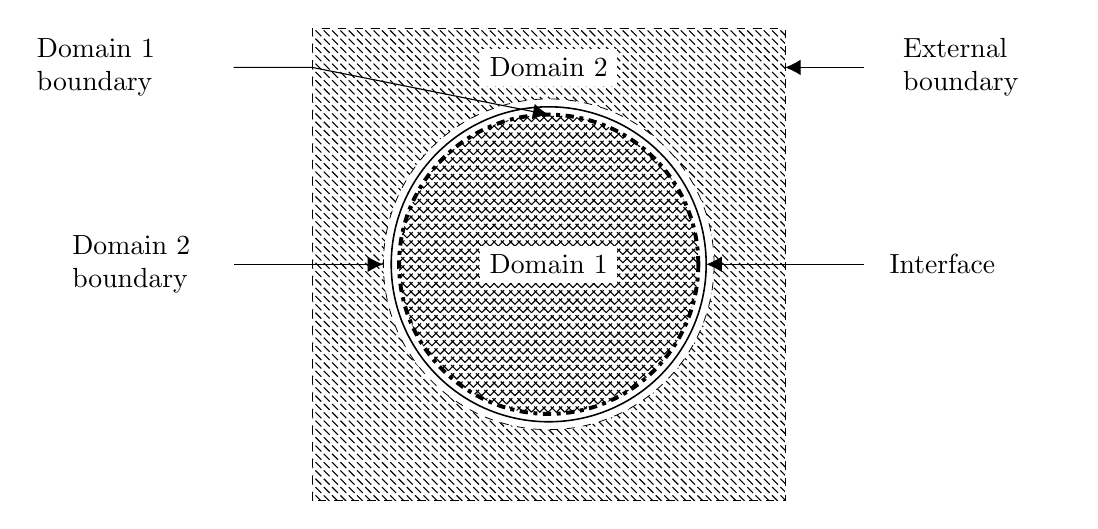
\begin{tikzpicture}
    \draw[pattern=north west lines,line width=0.1mm, dashed] (-3, -3) rectangle (3cm,3cm);
    \draw[fill=white, line width=0.1mm, dashed](0,0) ellipse (2.1cm and 2.1cm);
    \draw[line width=0.2mm](0,0) ellipse (2cm and 2cm);
    \draw[pattern=crosshatch, line width=0.5mm, dash dot](0,0) ellipse (1.9cm and 1.9cm);
    \node[fill=white] at (0, 0) {Domain 1};
    \node[fill=white] at (0, 2.5) {Domain 2};
    \draw[<-] (2, 0) -- node[xshift=2cm]{Interface}(4, 0);
    \draw[<-] (-2.1, 0) -- node[xshift=-2cm, text width=2cm]{Domain 2 \\ boundary}(-4, 0);
    \draw[<-] (0, 1.9) -- (-3, 2.5) -- node[xshift=-2cm, text width=2cm]{Domain 1 \\ boundary}(-4, 2.5);
    \draw [<-] (3.0, 2.5) -- node[xshift=2cm, text width=2cm] {External \\ boundary}(4.0, 2.5);
  \end{tikzpicture}
  }
  \caption{Schematic for the Coupled packing algorithm. The external region is
    marked as domain 2 and the internal region is marked as domain 1.}
  \label{fig:coupled}
\end{figure}

\begin{algorithm}[h!]
  \SetAlgoLined
  \KwResult{Coordinates of solids and fluids}
  \code{ReadInput()}\;
  \code{DivideDomain()}\;
  \code{CreateParticles()}\;
  \code{SetConstantAndTimeStep()}\;
  \code{Algorithm}\ref{alg:jiang0}\code{(domain1, 5000)}\;
  \code{Algorithm}\ref{alg:jiang0}\code{(domain2, 5000)}\;
  \code{iteration = 0}\;
  \code{converged = False}\;
  \While{\codek{not converged}}{
    \code{UpdateNeighbors(domain1 + domain2)}\;
    \code{ComputeAccelerations()}\;
    \code{IntegrateParticles()}\;
    \code{converged = CheckConvergence()}\;
    \code{iteration++}\;
  }
  \code{SeparateParticles()}\;
  \caption{Coupled particle packing algorithm.}
  \label{alg:jiang}
\end{algorithm}

\citet{jiang2015blue} have not specified a way to choose the value of the
constants in \cref{eq:backgrounpressure_jiang} and \cref{eq:coh}. We
heuristically choose the values of $\gamma=20$, $p_{b}=10$ and $h=\Delta s$
for all the simulations.

We note that there is no exterior defined in \cite{jiang2015blue}. In this
work, we pack the exterior in the same manner as the interior by moving the
boundary surface by $\Delta s/2$ and $-\Delta s/2$ for exterior and interior,
respectively. In \cref{fig:coupled}, we enclose the interior domain (domain
1) within a thick dashed line, and the exterior is within a thin dashed line
(domain 2). We represent each domain with a different pattern. Domain 2,
having an external boundary, has frozen particles outside it. The solid line
represents the boundary surface.

\begin{sloppypar}
We pack the particles in two different passes as described in algorithm
\ref{alg:jiang}. First, we read the geometry data in \code{ReadInput}
followed by particle initialization in \code{CreateParticles}. We divide the
free particles into domain 1 and domain 2 depending upon their location in
\code{DivideDomain}. We do the following for particles that are lying in
between the two dashed boundaries of domains 1 and 2. If a particle is in the
exterior region (outside the boundary surface), we move it along the normal
by a distance $\Delta s$ into domain 2. Similarly, we move particles between
the boundary surface and the domain 1 boundary into domain 1.
\end{sloppypar}

\begin{sloppypar}
  In the first pass, we solve domains 1 and 2 separately using the algorithm
  \ref{alg:jiang0}. In this case, each domain is unaware of the other. We
  perform the boundary particle projection onto the dashed lines of the
  respective boundaries. We move the particles in both the domains for a
  predetermined number of iterations, at which point the particles reach
  equilibrium\footnote{We choose the predetermined iterations to be 5000 based
    on the test cases considered.}. This step ensures that we sort all
  particles as either interior or exterior and have an interface which they
  cannot cross i.e.\ the dashed lines.
\end{sloppypar}

\begin{sloppypar}
In the second pass, when the projection is complete, we constrain the
particles on the interior surface i.e.\ the thick dashed line, to move along
it. We allow all other particles to freely move using
\cref{eq:backgrounpressure_jiang} in \code{ComputeAccelerations} and
\code{IntegrateParticles}. The iteration continues until the convergence
criteria in \code{CheckConvergence} as discussed in \cref{subsec:conv} is
satisfied. The presence of exterior particles eliminates the need for the
cohesion force; thus, we do not evaluate it once domains 1 and 2 starts
interacting. Using this approach, we obtain a uniform distribution both
inside and outside the surface. We note that the original implementation was
used to sample blue noise and does not require external particles.
\end{sloppypar}

We implement the proposed algorithms in the open-source SPH framework, PySPH
\cite{pysph2020}. The current implementation is open source and freely
available with this manuscript at \url{https://gitlab.com/pypr/sph_geom}. All
the results shown in the next section are fully reproducible using an
automation framework~\cite{pr:automan:2018}.


\section{Results and discussion}
\label{sec:results}
%
In this section, we compare all the algorithms discussed above. We first
compare the algorithms for a circular cylinder and a Z-shaped wall in two
dimensions. The Standard method is limited to two-dimensional domains and so
in three-dimensions we compare only the Coupled and the Hybrid method for an
ellipsoid. We also show the particle distribution for a symmetric airfoil and
an arbitrarily shaped geometry using the Hybrid method at different
resolutions. In the end, we demonstrate the Hybrid algorithm for a
complex-shaped Stanford bunny.

\subsection{Circular cylinder}
\label{sec:cyl}

\begin{figure}[htbp]
  \centering
  \includegraphics[width=\textwidth]{figures/cylinder_2d/cylinder_2dp_sf}
  \caption{Solid (Red) and fluid (Blue) particles for a circular cylinder for $\Delta s = 0.1$. }
  \label{fig:cyl_sf}
\end{figure}

\begin{figure}[htbp]
  \centering
  \includegraphics[width=\textwidth]{figures/cylinder_2d/cylinder_2d_p}
  \caption{Density distribution of the packed particles for the circular
    cylinder geometry for $\Delta s = 0.1$.}
  \label{fig:cyl_rho}
\end{figure}

\begin{figure}[ht!]
  \begin{subfigure}{0.5\textwidth}
    \centering
    \ifthenelse{\showimages=1}
    {
    \includegraphics[width=\textwidth]{figures/cylinder_2d/cylinder_2d_conv}
    }{}
    \caption{Function}
    \label{fig:cyl_f}
  \end{subfigure}
  \begin{subfigure}{0.5\textwidth}
    \centering
    \ifthenelse{\showimages=1}
    {
    \includegraphics[width=\textwidth]{figures/cylinder_2d/cylinder_2d_conv_df}
    }{}
    \caption{Derivative}
    \label{fig:cyl_df}
  \end{subfigure}
  \caption{$L_2$ error for SPH approximation of function and its derivative
    for the circular cylinder geometry.}
  \label{cyl_f_df}
\end{figure}

The flow of an incompressible fluid past a cylinder is a well-known benchmark
problem. In order to obtain a good results it is important to remove the
effect of any surface irregularities due to the underlying method of geometry
creation. In this test case, we compare the circular cylinder constructed
using all the approaches discussed in \cref{sec:alg}. We consider a cylinder
of diameter $D=2m$. In \cref{fig:cyl_sf}, we show the geometry with particle
spacing $\Delta s = 0.1$ constructed using different methods. It is clear that
the Hybrid method produces a uniform particle distribution. In the case of the
Coupled method, we observe a large number of particles near the wall surface.
The Standard method seems to have uniform particles owing to its construction.
In order to investigate this further, we plot the density distribution as
shown in \cref{fig:cyl_rho}. We obtain the density distribution using the
well-known summation density. Clearly, the Coupled method shows high density
near the surface, and the Standard method shows a low density on the solid
since we assume $\Delta s$ particle distance over a curved surface. The total
density variation is 8\%, 16\%, and 2\% for the Standard, Coupled, and Hybrid
methods, respectively. Thus, it is clear that the proposed Hybrid method shows
excellent distribution with a maximum variation of $2\%$.

We study the improvement quantitatively by interpolating a $C_{\infty}$
function over the packed particles given by
\begin{equation}
  f(x, y, z) = \sin(x^{2} + y^{2} + z^{2}).
\end{equation}
We approximate the function and its derivative using
\begin{equation}
  \left<f(\ten{x}_i)\right> = \sum_j f(\ten{x}_j) W_{ij} \frac{m_j}{\rho_{j}}
  \label{eq:sph_func}
\end{equation}
and
\begin{equation}
  \left<f_{x}(\ten{x}_i)\right> = \sum_j f(\ten{x}_j) W_{ij, x} \frac{m_j}{\rho_{j}},
  \label{eq:sph_derv}
\end{equation}
respectively. We evaluate the $L_2$ error in the approximation using
\begin{equation}
  L_2(f-f_{o}) = \sqrt{\frac{\sum_j (f(\ten{x}_j) - f_{o}(\ten{x}_j))^{2}}{N}}
  \label{eq:l2}
\end{equation}
where $f_o$ is the SPH function approximation on a regular mesh of points, and
$N$ is the total number of particles in the domain. The value of the function
is set as per the position of each particle as $f(\ten{x}_i)$. This is then
interpolated onto a regular mesh using \cref{eq:sph_func,eq:sph_derv}. We do
the same for the regular points themselves to obtain the reference $f_o$ value
at each point. We vary the value of $h$ in order to get convergence. We choose
a value of $h/\Delta s=1.0$ for $\Delta s = 0.1$ and vary linearly to
$h/\Delta s=1.5$ for $\Delta s =0.02$. We use the quintic spline kernel for
the interpolation. When comparing the derivatives, we consider only the $x$
derivative. In \cref{fig:cyl_f} and \cref{fig:cyl_df}, we show $L_{2}(f -
f_{o})$ and $L_{2}(f^{\prime} - f_{o}^{\prime})$. In these plots, we do not
evaluate the errors near the center of the cylinder since they do not affect
the flow and also the Standard method performs poorly in this region. Hence,
the $L_2$ norm is evaluated only over the points where $r>0.45 \ D$ as this
allows for a fair comparison. It is clear that the Hybrid method shows a
significant order of magnitude improvement compared to both Coupled and
Standard methods. The Coupled method is slightly better than the Standard
method. The Standard method shows large errors due to the way in which we
represent the surface.

\subsection{Zig-Zag Wall}

\begin{figure}[ht!]
  \centering
  \includegraphics[width=\textwidth]{figures/zig_zag_2d/zig_zag_2dp_sf}
  \caption{Solids (Red) and fluids (Blue) for the zig-zag wall for $\Delta s = 0.05$.}
  \label{fig:zwall_p_sf}
\end{figure}

\begin{figure}[ht!]
  \centering
  \includegraphics[width=\textwidth]{figures/zig_zag_2d/zig_zag_2d_p}
  \caption{Density distribution for the zig-zag wall for $\Delta s = 0.05$.}
  \label{fig:zwall_p}
\end{figure}


\begin{figure}[ht!]
  \begin{subfigure}{0.5\textwidth}
    \centering
    \ifthenelse{\showimages=1}
    {
    \includegraphics[width=\textwidth]{figures/zig_zag_2d/zig_zag_2d_conv}
    }{}
    \caption{Function Approximation}
    \label{fig:zz_f}
  \end{subfigure}
  \begin{subfigure}{0.5\textwidth}
    \centering
    \ifthenelse{\showimages=1}
    {
    \includegraphics[width=\textwidth]{figures/zig_zag_2d/zig_zag_2d_conv_df}
    }{}
    \caption{Derivative Approximation}
    \label{fig:zz_df}
  \end{subfigure}
  \caption{$L_2$ error for SPH approximation of function and its derivative for the zig-zag wall.}
\end{figure}

The zig-zag wall is one of the test cases proposed by
\citet{marrone-deltasph:cmame:2011} used to demonstrate the $\delta$-SPH
method. They employ the Standard packing algorithm in order to generate a
solid body and pack the fluid particles around. In this test case, we pack
particles using all the algorithms and compare the density and function
approximations as done earlier. The zig-zag wall is an excellent test case for
packing since it has both concave and convex sharp edges. In order to generate
a solid using the Standard method, we move the corner nodes along the angle
bisector and generate uniform points using these points as endpoints. In the
other two algorithms, we refer to these sharp points as corner nodes, and
employ the method discussed in \cref{subsec:pm} to automatically restrict the
motion of these points.

In \cref{fig:zwall_p_sf}, we show the solid and fluid particles packed with
$\Delta s=0.05$ using different algorithms. It is difficult to conclude which
of these is better. However, on looking at the density distribution computed
using the summation density as shown in \cref{fig:zwall_p}, the proposed
method has much less deviation from the desired density. In the case of the
Coupled method, we observe higher density at the concave corner. This
increase occurs since the particles from both sides push towards the
interface at the first pass of the Coupled algorithm as discussed in
\cref{sec:jiang}. The Standard method shows an uneven variation of density
near the sharp edges, which is not desirable. The total density variation is
10\%, 30\%, and 3\% for Standard, Coupled, and Hybrid methods, respectively.
It clearly shows that the Hybrid method shows very small density variations
compared to other methods.

We perform a similar analysis over the zig-zag wall as done in the case of
the cylinder. In order to remove the effect of the interior of the solid in
the standard case, we compute the errors only up to a distance of $\Delta s$
inside the wall. In \cref{fig:zz_f} and \cref{fig:zz_df}, we plot the $L_2$
norm for the error in function and its derivative SPH approximation,
respectively. Clearly, the proposed method performs very well as compared
with the other methods.


\subsection{Packing at different resolutions}
\label{sec:resol}

In this example, we apply the Hybrid algorithm to an arbitrarily shaped body.
We show the packing at different particle spacings in \cref{fig:arb_part}.
The particle spacings chosen are $0.05$, $0.075$, and $0.1$. We place the
particles at $\Delta x /2$ distance away from the boundary. Clearly, the
density distribution is close to the desired value of $1.0$. The particles
conform to the body surface and have a total variation of density of $2.5\%$,
$2\%$, and $3\%$ for particle spacing $0.1$, $0.075$, and $0.05$,
respectively. It shows that the proposed algorithm is applicable to complex
two-dimensional geometries.

\begin{figure}[ht!]
  \centering
  \ifthenelse{\showimages=1}
  {
    \includegraphics[width=0.45\textwidth]{{figures/arbitrary_object_2d/arbitrary_object_2dnx_0.1}.png}
    \includegraphics[width=0.45\textwidth]{{figures/arbitrary_object_2d/arbitrary_object_2dnx_0.075}.png}
    \includegraphics[width=0.45\textwidth]{{figures/arbitrary_object_2d/arbitrary_object_2dnx_0.05}.png}
  }{}
  \caption{Density distribution at different resolutions for an arbitrary shaped object.}
  \label{fig:arb_part}
\end{figure}


\subsection{Effect of convergence tolerance on the quality}
\label{sec:tol}

\begin{sloppypar}
This test case shows that the proposed algorithm can achieve a
high-quality particle distribution for a given tolerance. We consider a
symmetric airfoil, NACA0015. We choose the endpoint at the trailing edge as a
corner node. We perform particle packing using the proposed Hybrid method for
the spacing $\Delta s= 0.02$.
\end{sloppypar}

In \cref{table:tol}, we tabulate the number of iterations required for
convergence and the $L_{\infty}$ error in the density for different values of
the tolerance required for convergence. It is evident from the table that the
$L_{\infty}$ error decreases with the decrease in the tolerance; however, the
number of iterations required increases significantly. In the
\cref{fig:airfoil}, we show the high-quality particle distribution achieved
using a lower value of tolerance, $\epsilon=2.5\times 10^{-5}$. It shows that
the proposed method can achieve a high-quality particle distribution provided
we use a sufficiently low tolerance.

\begin{table}[h!]
  \centering
  \input{figures/convergence_test/tol}
  \caption{The table shows the effect of the change in tolerance for
  convergence on the number of iterations and the $L_{\infty}$ error in the
  density.}
  \label{table:tol}
\end{table}

\begin{figure}[ht!]
  \centering
  \includegraphics[width=0.7\textwidth]{{figures/convergence_test/convergence_testtol_0.0025}.png}
  \caption{The density distribution for a symmetric airfoil with particle
  spacing, $\Delta s=0.02$ and convergence tolerance, $\epsilon=2.5 \times 10^{-5}$.}
  \label{fig:airfoil}
\end{figure}


\subsection{Particle Packing in 3D}

\begin{figure}[ht!]
  \begin{subfigure}{0.5\textwidth}
    \centering
    \ifthenelse{\showimages=1}
    {
    \includegraphics[width=\textwidth]{{figures/sphere/new_dx_0.1}.png}
    }{}
    \caption{Hybrid}
    \label{fig:sph2}
  \end{subfigure}
  \begin{subfigure}{0.5\textwidth}
    \centering
    \ifthenelse{\showimages=1}
    {
    \includegraphics[width=\textwidth]{{figures/sphere/jiang_dx_0.1}.png}
    }{}
    \caption{Coupled}
    \label{fig:sph1}
  \end{subfigure}
  \caption{Density distribution on the surface of the ellipsoid for $\Delta s = 0.1$.}
  \label{fig:sphere_part}
\end{figure}

\begin{figure}[ht!]
  \begin{subfigure}{0.5\textwidth}
    \centering
    \ifthenelse{\showimages=1}
    {
    \includegraphics[width=\textwidth]{{figures/sphere/sphere_conv}.png}
    }{}
    \caption{Function approximation}
    \label{fig:sphere_f}
  \end{subfigure}
  \begin{subfigure}{0.5\textwidth}
    \centering
    \ifthenelse{\showimages=1}
    {
    \includegraphics[width=\textwidth]{{figures/sphere/sphere_conv_df}.png}
    }{}
    \caption{Derivative  approximation}
    \label{fig:sphere_df}
  \end{subfigure}
  \caption{$L_2$ error for SPH approximation of function and its derivative for the ellipsoid.}
  \label{fig:sphere_f_df}
\end{figure}
One of the advantages of the proposed algorithm is that it can be easily
extended to a three-dimensional object, unlike the Standard method. In order
to compare the packing in 3D, we pack particles for a simple ellipsoid. The
ellipsoid has semi-major axis dimensions, $a=1.0$, $b=0.5$ and $z=0.75$ along
$x$, $y$ and $z$ axis, respectively. In \cref{fig:sph2} and \cref{fig:sph1},
we show the packed particles over the surface of the sphere for the Hybrid
and Coupled method, respectively. The color of the particles shows the
density distribution. In order to show that the particles conform to the
surface, we pull the surface along the normal by $\Delta s/2$. It is clear
that the Hybrid method attains a good distribution of particles resulting in
a density distribution very close to $\rho_{o}=1.0$. The particle
distribution using the Coupled method has density near the lower range of the
scale. It is due to the fact that, unlike the Hybrid method, the Coupled
method does not project the required number of particles on the surface. In
order to perform a quantitative analysis, we adopt the comparison of the
function and derivative approximation used earlier. In \cref{fig:sphere_f}
and \cref{fig:sphere_df}, we plot $L_2$ error in SPH approximation of
function and its derivative, respectively. As can be seen, the proposed
method produces much lower errors at lower resolutions.

\begin{figure}[ht!]
  \centering
  \includegraphics[width=0.45\textwidth,trim={3cm 0 4.5cm 1.5cm},clip]{figures/bunny/bunny_1}
  \includegraphics[width=0.45\textwidth, trim={3cm 0 4.5cm 1.5cm},clip]{figures/bunny/bunny_2}
  \includegraphics[width=0.6\textwidth]{figures/bunny/bunny}
  \caption{Different views showing particles (colored with density values)
    over the Stanford bunny.}
  \label{fig:bunny}
\end{figure}

In order to show the capability of the algorithm, we also apply the proposed
algorithm to the Stanford bunny geometry, as done by \citet{jiang2015blue}.
The geometry surface must have outward normals, and we correct the
mesh using a mesh manipulation tool. We choose a particle spacing of $0.02$.
In this case, the intention is to show how well we capture the geometry so
we do not shift the surface inside. In \cref{fig:sph1}, we show the particle
distribution over the surface of the bunny. The results show the
applicability of the proposed algorithm to arbitrary-shaped 3D objects. After
pre-processing, we can place the 3D object anywhere in the domain with the
surrounding particles.


\section{Conclusions}
\label{sec:conclusions}

This paper proposes an improved particle packing algorithm to simulate flows
involving complex geometries in two and three dimensions. We implement and
compare three different methods for packing particles around an
arbitrary-shaped object namely, (i) the Standard method proposed by
\citet{colagrossi2012particle} along with the solid object construction
proposed by \citet{marrone-deltasph:cmame:2011}, (ii) the Coupled method, a
modified version of that proposed by \citet{jiang2015blue}, handles both the
interior and exterior of the body, and (iii) a new method that combines the
best features of these methods. The proposed method provides an excellent
density distribution as a result of evenly distributed particles. The method
applies to both 2D and 3D domains. Unlike the Coupled method, we do not
require estimation of particles inside and outside. We show several benchmark
cases which highlight the accuracy of the proposed algorithm in two and three
dimensions. We provide an open-source implementation of the manuscript, and
the manuscript is fully reproducible.

The SPH method is being applied to a wide variety of problem domains involving
complex geometries. While mesh-free particle methods do not require a mesh,
one must still capture the boundaries accurately. However, there are not many
tools to create good quality initial particle distributions. This is necessary
for accurate simulation of incompressible fluid flows with the SPH. The
proposed method is largely automatic and offers researchers the ability to
easily discretize complex geometries using particles in two and three
dimensions. Since we construct the proposed algorithm using ideas from SPH, it
should be easy to incorporate into an SPH solver. The code is also
open-source, and hence researchers could also choose to use our
implementation.

In the future, we plan to make it easier to use and also integrate with the
main PySPH package. We have only demonstrated our implementation on the CPU.
However, PySPH supports execution on a GPU, and we plan to make the necessary
modifications for efficient execution on the GPU. The method currently works
best for a fixed resolution. In the future, it would be helpful to explore
this in the context of adaptive resolution.


\section*{References}
\bibliographystyle{model6-num-names}
\bibliography{references}


\end{document}

%%% Local Variables:
%%% mode: latex
%%% TeX-master: "paper"
%%% fill-column: 78
%%% End: